\documentclass[../thesis.tex]{subfiles}

\begin{document}


\section{Overview}
In this final chapter, we aim to target the questions motivating Chapter~\ref{chap:tmb_estimation} in their broader context. In particular, previously we have relied on an established body of literature verifying the utility of \gls{tmb} as a proxy biomarker for response to immunotherapy. This has been advantageous in that is has allowed us not to concern ourselves with directly showing our derived mutation signatures are associated with improved response to immunotherapy (aside from in some particular cases, such as in Figure~\ref{fig:responseclass}). Indeed, in Chapter~\ref{chap:tmb_estimation} we have been able to leverage datasets that did not provide information on response to treatment with immunotherapy. Instead, we've simply aimed to predict \gls{tmb} as well as we can from targeted panel data (often `artificial' panel data derived from \gls{wes}). This has been especially convenient because \gls{tmb} can be directly calculated from \gls{wes} data and does not needed to be provided by a study as a separate covariate.  While aiming to predict \gls{tmb} has been a helpful simplification, broader methods are required if we wish to more directly interrogate the relationship between genomic signatures (including but not limited to \gls{tmb}) derived from targeted sequencing and clinical outcomes. Here we discuss in detail strategies for causal estimation of treatment effect on survival from observational studies, a relatively new field. We review some basics of survival analysis and causal inference, describe some recent developments in combining the two, and briefly demonstrate two very different methodological approaches on targeted sequencing data. These examples, rather than focusing on the results derived, serve as an opportunity to discuss advantages and disadvantages of different approaches.

\section{Introduction}

In order to more fully understand the relationship between somatic biomarkers such as \gls{tmb} and clinical outcomes, two substantial hurdles are presented. Firstly, while in Chapter~\ref{chap:tmb_estimation} we were able to utilise two small datasets for which binary clinical outcomes (corresponding to `durable clinical benefit') were available, in general the measurement of clinial outcomes is not as simple. By far the most common means of reporting is via survival-like clinical outcomes. These can track a variety of endpoints, such as \glsfirst{os} or \glsfirst{pfs}, but are fundamentally restricted by the timespan of a given study period such that not every sample has an associated endpoint observed. This problem is known as \textit{censoring} and is discussed in Section~\ref{sec:survival}. Secondly, our reliance on \gls{tmb} was motivated by extensive work establishing \gls{tmb}'s clinical utility in randomised treatment scenarios. We often don't have the resources to conduct a large \gls{rct}, and so will have to proceed by combining multiple \emph{observational} datasets. This requires a framework for causal inference, and the one we choose is known as \glsfirst{hte}, described in Section~\ref{sec:hte}\footnote{Note that there is no reason causal analysis techniques cannot be applied to experimental data such as derived from \glspl{rct}, but in analysing observational data they are necessary.}.

In this chapter, after describing the fundamentals of survival analysis (Section~\ref{sec:survival}) and \gls{hte} (Section~\ref{sec:hte}) we review recent literature on methods to combine these two techniques in Section~\ref{sec:hte_survival}. In Section~\ref{sec:immuno_hte}, we briefly demonstrate an application of these methods to verify the causal role of \gls{tmb} by combining two somatic mutation datasets, and then discuss applying them to produce more flexible estimators of benefit from immunotherapy.

\section{Survival analysis \label{sec:survival}}


\subsection{Survival times}
Survival analysis concerns modelling the amount of time elapsing before a given event occurs. In medical settings, this is often time-to-death analysis, but the same framework is used to approach other events, both medical (e.g. relapse or visit to hospital) and non-medical (machine lifetime, customer churn, etc.). Since our main application cases are concerned with \gls{os}, we will refer here to a generic `event' as death. For a patient $i$, we will refer to survival times with either a lower case $t_i$ (for observations) or upper case $T_i$ (for random variables). As a starting point for motivating techniques in survival analysis, we note the following properties we might expect from survival times:
\begin{enumerate}
    \item Survival times are \emph{continuous}: $t_i \in \mathbb{R}$. This is intuitively true in many situations, but we typically only measure data in discrete bins (e.g. months). This can introduce complexities such as exact ties in survival time.
    \item Survival times are \emph{positive}: $t_i > 0$. This is a consequence of survival times always being {relative to some other time point}. The choice of this baseline can often vary between (and even within) studies.
\end{enumerate}
The second point above emphasises the importance of an appropriate definition of starting time for interpreting survival times. Defining suitable end points can also present nuanced issues, particularly accounting for, for example, deaths due to competing risks. While this is studied extensively in the literature, in this work we assume a fairly simple modelling scenario with no patients removed from the dataset from external causes. One form of removal/missingness that we certainly do care about, however, is \emph{censoring}. 

\subsection{Censoring}
Censoring refers to a structured pattern of non-observance of a given outcome, in this case, the death of a patient. In the studies we will discuss in this chapter, this is typically because the period of observation for the study ended. This is know as \emph{right}-censoring. Because we have not observed the death of the patient, we only have access to a one-sided interval in which this would have occurred. Addressing censoring is one of the core missions of survival analysis.

At this point we introduce some notation. For a patient $i$, we let $c_i \in \mathbb{R}^{+}$ (or $C_i$ for a random variable) denote the time at which the patient is removed from further observation, relative to the baseline observation time point for that patient. We therefore observe only the following: $y_i \in \mathbb{R}^{+}$ (or $Y_i$ for random variable) is the time of final follow-up, i.e. $y_i = \min(c_i, t_i)$; and $\delta_i$ (or $\Delta_i$) for censorship status, i.e. $\delta_i = \mathbbm{1}\{t_i \leq c_i\}$. 

Our general aim, therefore, is to perform inference about the behaviour of the random variables $T_i$ from observation only of a given set of $n$ pairs $\{(y_i, \delta_i)\}_{i=1}^{n}$. Here we assume that these tuples of observations (and potential future observations) are realisations of independent and identically distributed random variables, and so refer to this underlying joint distribution without reference to sample $i$, i.e. we may consider the joint variable ($T, C, \Delta)$.  We discuss in the next section some common practices for performing inference on these targets.

One further concept worth mentioning is that of \emph{informative} vs \emph{non-informative censoring}. In the latter, it is assumed that censoring is independent of survival time, given the covariates. Throughout this chapter, we assume we are considering non-informative censoring for simplicity, although some of the methods presented have mechanisms for adjusting for informative censoring (see for example the CSA-INFO method of \citealp{chapfuwa_enabling_2021}).
   
\subsection{Modelling approaches} \label{sec:survival_modelling}
We now describe some common approaches to statistical modelling of survival data. We begin by defining \textit{hazard}. While it is possible to characterise the distribution of survival times $T$ in a variety of ways, hazard is common as it is both interpretable and easy to work with. For the distribution $T$, we define hazard $h(t)$ as a function of time $t$ as the instantaneous rate of death at time $t$, given survival up until time $t$, via:
\[
    h(t) := \lim_{\delta t \rightarrow 0} \frac{\mathbb{P}(T \in [t, t + \delta t] | T > t)}{\delta t}.
\]
We also define the \textit{survival} function $S(t)$ as $\mathbb{P}(T > t)$. We may then observe that hazard is expressible as 
\begin{align*}
    h(t) & = \lim_{\delta t \rightarrow 0} \frac{\mathbb{P}(T > t) - \mathbb{P}(T > t + \delta t)}{\mathbb{P}(T > t) \delta t} \\
    & = \frac{1}{S(t)} \lim_{\delta \rightarrow 0} \frac{S(t) - S(t + \delta t)}{\delta t} = - \frac{1}{S(t)} \frac{d}{dt} S(t)\\
    & = - \frac{d}{dt} \log S(t). 
\end{align*}
Finally note that $\frac{dS}{dt} = - f(t)$, where $f(t)$ is the probability density function for $T$, so we may also write $h(t) = \frac{f(t)}{S(t)}$. This is consistent with the intuition that hazard denotes rate of death, scaled by likelihood of survival so far. Often when fitting predictive models, we use hazard as the target of prediction given inputs $x$, aiming to estimate $h(t|x)$. Before we move on to this case, however, we'll discuss a few more properties of hazard. It can be useful to define the cumulative hazard function $H(t) = \int_{0}^{t}h(u)du$. We can then write down further useful relations between hazard, cumulative hazard, and density. Firstly note that 
\begin{align*}
H(t) & := \int_{0}^{t}h(u)du \\
& = -\int_{0}^{t}\frac{d}{du} \big(\log S(u)\big) du  = - \big[\log S(u) \big]_{0}^{t}  = -\log S(t),
\end{align*}
so we can also express $H(t)$ in terms of the survival function. Likewise we can express $f(t)$ simply in terms of hazard via
\[ f(t) = h(t)S(t) = h(t)\exp (-H(t)).\]
From this last relationship we can quickly see that under an assumption of \emph{constant hazard} $h(t)=\lambda$, survival times will follow an exponential distribution, with density function $f(t) = \lambda \exp(-\lambda t)$, with mean $\lambda^{-1}$ and variance $\lambda^{-2}$.

However, as mentioned above, a single model for all survival times is not sufficient for most purposes. In general we want to learn about the effect of some covariates on survival time. We therefore introduce a random (potentially vector-valued) variable $X$ taking values in $\mathbb{R}^p$, and define the following conditional versions of survival and hazard functions:
\begin{align*}
    h(t|x) & := \lim_{\delta t \rightarrow 0} \frac{\mathbb{P}(T \in [t, t + \delta t] | T > t, X = x)}{\delta t} \\
    S(t|x) & := \mathbb{P}(T > t | X = x).
\end{align*}
Note that the same relationships as above hold. When making decisions around modelling, assumptions about the behaviour of these two functions are typically the starting point. We'll here evaluate two common assumptions, based on restricting the functional form of each of these two functions respectively.

\subsubsection{The proportional hazards assumption}
Proportional hazards models are based on the assumption that changes in a given covariate have the effect of increasing hazard by a constant factor across all time points. We state this formally as follows: that there exist functions $h_0: \mathbb{R}^+ \rightarrow \mathbb{R}^+$ and $\theta: \mathbb{R}^p \rightarrow \mathbb{R}^+$ such that 
\[h(t|x) = h_0(t) \theta(x). \]
In practice the function $\theta$ is often chosen to be $\theta(x) = \exp (- \beta^T x)$ for parameter $\beta \in \mathbb{R}^p$ to be fitted. In this case $h_0(t)$ is left to be fitted flexibly (although this is not necessary for inferring $\beta$, making the resulting model (the Cox model; \citealp{cox_regression_1972}) semi-parameteric. Note that we can derive the resultant form of the survival function as $S(t|x) = S_0(t)^{\theta(x)}$, where $S_0(t) = \exp(-\int_{0}^{t}h_0(u)du)$.


\subsubsection{The accelerated failure time assumption}
Accelerated failure time models \citep{wei_accelerated_1992} are based on the assumption that changes in a given covariate have the effect of scaling the entire lifetime of a patient by a constant factor. This is formalised by position that there exist functions $S_0: \mathbb{R}^+ \rightarrow [0,1]$ and $\theta: \mathbb{R}^p \rightarrow \mathbb{R}^+$ such that 
\[S(t|x) = S_0(\theta(x)t).\]
As for proportional hazards, the function $\theta$ is often chosen to be $\theta(x) = \exp (-\beta^T x)$. Again as above, we may use this restriction to infer the form of the hazard function as $\theta(x)h_0(\theta(x)t)$, where $h_0(t) = -\frac{d}{dt} \log S_0(t)$. The function $S_0(t)$ is often chosen to be the exponential survival function $e^{-t}$.

Note that the proportional hazards and accelerated failure time assumptions are not mutually exclusive. Consider for example the following setting: $T$ is Weibull distributed with parameters $\lambda, k$, i.e. has cumulative distribution function $1- \exp((t/\lambda)^k$. Now suppose that the parameter $\lambda$ is given by $\lambda = \lambda_0 \exp(\beta^T x)$. We then have that 
\[S(t|x) = \exp\big(-t^k\lambda_0^{-k}\exp( -\beta^Tx)\big), \]
which satisfies the correct form for the accelerated failure time assumption with $S_0(t) = \exp(-t^k)$ and $\theta(x) = \lambda_0^{-k}\exp(\beta^Tx)$. We can also show that the hazard is given by 
\[h(t|x) = kt^{k-1}\lambda_0^{-k} \exp(-k\beta^Tx), \]
satisfying the proportional hazards assumption with $h_0(t) = k\lambda_0^{-k}t^{k-1}$ and $\theta(x) = \exp(-k\beta^Tx)$. 



\subsection{Fitting survival models}

\paragraph{The Cox proportional-hazards model}
The Cox proportional-hazards models \citep{cox_regression_1972} remains by far the most commonly employment survival analysis techniques, and represents once of the most significant contributions to statistics of the twentieth century. As would be expected, Cox regression employs the proportional hazards assumption described in the previous section in a semi-parametric linear model of the hazard function. The Cox model can be stated as follows:
\[h(t|x) = h_0(t) \exp(x^T\beta). \]
In the language of Section~\ref{sec:survival_modelling}, we refer to $\theta(x) = \exp(x^T\beta)$ as the `parametric' portion of the model (parameterised by the vector $\beta \in \mathbb{R}^p$), while the \emph{baseline hazard} function $h_(t)$, when needed, is typically fitted with non-parametric methods. The term semi-parametric is used to describe the combination of these two components. However, the power of Cox regression is that the parameter $\beta$ can be inferred without the need to fit the non-parametric baseline hazard $h_0(t)$. This is achieved via minimisation of the partial likelihood:
\[\mathcal{L}(\beta) = \prod_{i:\delta_i=1} \frac{\exp(x_i^T\beta)}{\sum_{j: t_j \geq t_i}\exp(x_j^T\beta)},\]
which can be separated from all non-parametric estimates of the model and used as an objective for minimisation with respect to $\beta$.

\paragraph{Non-parametric methods} \label{sec:nonparametric}
While Cox proportional hazards models are by far the most commonly applied methodology underlying the majority of survival analyses, the specific nature of the Cox partial likelihood is not always easy to adapt to scenarios where more flexible survival distributions are sought. This is not to say that the regression function underlying a Cox model cannot be more general; indeed, methods such as \emph{DeepSurv} \citep{katzman_deepsurv_2018} have made use of deep neural networks to specify a proportional hazards function. However, even in this scenario the proportional hazards assumption can be quite restrictive. Later in this chapter we demonstrate a method for non-parametric survival analysis due to \citet{chapfuwa_adversarial_2018}. Their strategy relies on applying a flexible regression function to a known source of simple randomness (e.g. a neural network applied to a multivariate normal source). To fit such models, they propose a loss function that includes an optimisation term to ensure that predicted survival times are \emph{a)} close to true survival times in the case of uncensored data and \emph{b)} greater than the observed censoring time in the case of censored data. To be specific, for a predicted survival time $t$, observed endpoint time $y$ and censoring status $\delta$ they penalise their loss function with 
\[\delta |t-y| + (1-\delta)\max\{0, y - t\}. \]
Here we see the first term (applied to uncensored data) penalises estimated survival times far from the observed value, and the second term (applied to censored data) penalises estimated survival times less than the observed censoring time. In their original paper \citet{chapfuwa_adversarial_2018} propose weighting these terms in a tunable manner, while in later work (such as applied to \gls{hte} estimation in \citealp{chapfuwa_enabling_2021}) they present them without tuning parameters. 


\section{Causal inference and heterogeneous treatment effects \label{sec:hte}}
\Glsfirst{hte} estimation refers to the discovery of interactions between the effect of some intervention, or \emph{treatment}, and some other covariates. In particular we aim to predict, from some input covariates, the change in outcome for a given sample upon applying a given intervention, while by definition never being able to observe a sample when the given treatment has both been applied and not been applied (referred to as the \emph{fundamental problem for causal inference}; \citealp{holland_statistics_1986}). 

\subsection{Potential outcomes}
We first consider the following scenario:  a binary treatment indicator variable $A$ taking values in $\{0,1\}$,  covariates $X$ taking values in $\mathcal{X} \in \mathbb{R}^p$ (also sometimes referred to as \emph{confounders}), and a response variable $Y$ taking values in $\mathcal{Y}$. In this section we will assume that the space $\mathcal{Y}$ is simple (e.g. the space of binary outcomes $\mathcal{Y} = \{0,1\}$), while in later sections we will deal with situations in which $Y$ takes composite values as in a survival analysis. We want to understand the effect of altering the treatment $A$ on the outcome $Y$. A natural quantity to estimate might be
\[\bbE[Y | A = 1] - \bbE[Y | A = 0].\]
However, if both $Y$ and $A$ depend on $X$, we might observe some spurious dependencies. We therefore want to develop a framework in which we are comparing reasonable \emph{potential outcomes} of $Y$ in a hypothetical alternate universe in which we had intervened/not intervened to change $A$.

Let $Y^{(0)}, Y^{(1)}$ refer to potential outcomes taken by $Y$ under intervention with $A=0,1$
respectively. We may therefore say that $Y=Y^{(A)}$\footnote{In the alternate notation of do-calculus \citep{pearl_causal_1995, pearl_-calculus_2012}, we would say that $\mathbb{P}(Y^{(a)} = y) := \mathbb{P}(Y = y |  \text{do}(A=a))$.}. We make two further assumptions: 
\begin{enumerate}
    \item \emph{Positivity:} the propensity function is positive almost everywhere, i.e. 
    \[\pi(x) := \mathbb{P}(A=1 | X = x) \  \text{is such that} \ \pi(X) \in (0,1) \ \text{almost surely.}\]
    \item \emph{No unmeasured confounders:} treatment is `essentially random' given $X$, i.e.
    \[\{Y^{(0)}, Y^{(1)}\} \perp\!\!\!\perp A | X. \]
\end{enumerate}
These are considered sufficient to estimate the \emph{\gls{ate}}.

\subsection{Average treatment effect}
The \glsfirst{ate} is defined via $ATE := \bbE[Y^{(1)} -Y^{(0)}]$. The assumptions described in the previous section are sufficient for the \gls{ate} to be identifiable \citep{stone_assumptions_1993}, since 
\begin{align*}
    ATE & = \bbE[Y^{(1)} - Y^{(0)} ] & \\
    & = \bbE[\bbE[Y^{(1)} - Y^{(0)} | X]] & \text{(by the tower property)} \\
    & = \bbE[\bbE[Y^{(1)} | X]] - \bbE[\bbE[Y^{(0)} | X]] & \\ 
    & = \bbE[\bbE[Y^{(1)} | X, A = 1]] - \bbE[\bbE[Y^{(0)} | X, A = 0]] & \text{(by Assumption~2)} \\
    & = \bbE[\bbE[Y | X, A = 1] - \bbE[Y | X, A = 0]], & \label{eq:ate}
\end{align*}
and $X$, $Y$ and $A$ are all observed quantities. Assumption~1 establishes that we can expect to observe samples with both $A=0$ and $A=1$ across the support of $X$. Methods for estimation of $ATE$ have been proposed for a variety of modelling assumptions and contexts \citep{reiersol_confluence_1945, thistlethwaite_regression-discontinuity_1960, rosenbaum_central_1983, abadie_semiparametric_2005, craig_natural_2017, roth_whats_2023}. One common such method is propensity score matching, which relies on partitioning observations into groups with approximately equal propensity scores. Note that 
\begin{align*}
    \mathbb{P}(A=1 | \pi(X), Y^{(1)}, Y^{(0)}) & = \bbE[A | \pi(X), Y^{(1)}, Y^{(0)}]  \\
    & = \bbE[\bbE[A | X, Y^{(1)}, Y^{(0)}] | \pi(X), Y^{(1)}, Y^{(0)}] \\
    & \hspace{50pt} \text{(by the tower property)}\\
    & = \bbE[\bbE[A|X]|\pi(X), Y^{(1)}, Y^{(0)}] \\ & \hspace{50pt} \text{(by Assumption~2)} \\
    & = \bbE[\pi(X) | \pi(X), Y^{(1)}, Y^{(0)}] 
 \\ & \hspace{50pt} \text{(by definition of propensity)} \\
    & = \pi(X) = \mathbb{P}(A=1|\pi(X)), 
\end{align*}
so that $\{Y^{(0)}, Y^{(1)}\} \perp\!\!\!\perp A | X \Rightarrow \{Y^{(0)}, Y^{(1)}\} \perp\!\!\!\perp A | \pi(X)$ (this is due to \citealt{rosenbaum_central_1983}). We can then say that
\[ATE = \bbE[\bbE[Y|\pi(X), A=1] - \bbE[Y|\pi(X), A=0]].\]
To estimate the \gls{ate} we therefore need only to average over the marginal distribution of $\pi(X)$ rather than the entire marginal distribution of $X$, which can be particularly useful when $X$ is high-dimensional.

While it is often useful to gauge the utility of a treatment across an entire population via the ATE, it does not necessarily make any progress towards recommending whether treatment will benefit a given patient. For this, we need heterogeneous, conditional, or individual treatment effect, discussed in the following section.

\subsection{Treatment with covariates}
We now define \glspl{hte} (also referred to as 
\glsxtrlong{cate}), which will be our tool to make predictions at the individual level. We define the treatment function $\tau: \mathcal{X} \rightarrow \mathcal{Y}$ as follows:
\begin{align*}
    \tau(x) & := \bbE[Y^{(1)} | X =x] - \bbE[Y^{(0)} | X=x] \\
    & = \mu_1(x) - \mu_0(x) 
\end{align*}
where $\mu_a(x) := \bbE[Y^{(a)}|X=x]$ is the conditional regression function for potential outcome $A=a$. Note that the logic demonstrated in the derivation of the identifiability of the \gls{ate} applies to conditional treamtent effect and we can also say that (under Assumptions~1~and~2) we have that $\mu_a(x) = \bbE[Y|X=x,A=a]$. This means that one viable strategy for estimation of \glspl{hte} is simply to estimate $\mu_0,\mu_1$ with $\muhat_0, \muhat_1$ respectively, and $\tau$ with $\hat{\tau}(x) := \muhat_1(x) - \muhat_0(x)$. We will discuss this strategy, known as a $T$-Learner, and its potential shortcomings in the next section.

While we've introduced \glspl{hte} in order to be able to make decisions at the individual level, it is worth pointing out that it is in general distinct from individual treatment effect \citep{vegetabile_distinction_2021}. In essence, since heterogeneous effect only requires conditioning on some set of covariates satisfying the strong ignorability assumption, it need not contain all relevant information about $Y$. In particular, suppose we are given a variable $X$ satisfying strong ignorability. Then we can form $X'=(X,Z)$ for any other covariate $Z$ estimate an identifiable \glspl{hte}. To emphasise the difference between truly individual treatment effects and those based merely on conditioning on some strongly ignorable set of variables, some authors use the term \emph{\gls{cate}} \citep{vegetabile_distinction_2021}.

\subsection{Meta-learner strategies}
\label{sec:metalearners}
As mentioned in the above, we divide strategies for estimating \glspl{hte} into general classes of \emph{meta-learner} \citep{kunzel_metalearners_2019, curth_nonparametric_2021}. Each of these relies on some baseline strategy for fitting a regression function given a training dataset of inputs and outputs (e.g. linear regression, random forests, a neural network), and applies it to some combination of target functions. We describe a few below.

\begin{enumerate}
    \item \label{tech:tlearner} $T$-Learners: this base strategy centred on the identifiability of the conditional regression functions $\mu_0, \mu_1$. We simply split our dataset into two portions such that, according to observed values, the treatment variable takes the values $A=0$ or $A=1$. We then fit $\muhat_0(x), \muhat_1(x)$ separately on these two subsets, and define:
    \[ \hat{\tau}(x) := \muhat_1(x) - \muhat_0(x).\]
    \item $S$-Learners: a small variation on $T$-Learners. With this approach we jointly fit $\muhat(x,a)$ such that $\muhat(x,0) \approx \mu_0(x)$ and that $\muhat(x, 1) \approx \mu_1(x)$, then define:
    \[\hat{\tau}(x) := \muhat(x,1) - \muhat(x,0).\]
    \item \label{tech:ipw} Methods based on \emph{pseudo-outcomes} define some intermediate statistic that can be estimated based on observed data. The simplest is based on the Horvitz-Thompson transformation \citep{horvitz_generalization_1952}, also known as \gls{ipw}. We define:
    \[\Tilde{Y}_{IPW} := \Big(\frac{A}{\pihat(X)} - \frac{1-A}{1-\pihat(X)}\Big)Y, \]
    relying on the observation that, if $\pihat(x) = \pi(x)$, then $\bbE[\Tilde{Y}_{IPW} | X =x] = \tau(x)$. The advantage of this approach is that the quantity $\Tilde{Y}_{IPW}$ only depends on observable quantities, and so can be estimated from the full dataset.
    \item Hybrid methods comprise some combination of strategies based on fitting potential regression functions (for example via $T$-Learners) and pseudo-outcomes. These include $X$-Learners as proposed by \citet{kunzel_metalearners_2019} -- for which special cases have been investigated further by \citet{curth_nonparametric_2021} -- and generalised `doubly robust' estimators proposed by \citet{kennedy_optimal_2020}. In this context, double robustness refers to a learner that produces consistent estimates even if only one of $\muhat$ and $\pihat$ are correctly specified.
    \item \citet{nie_learning_2017} proposed an alternate hybrid method, termed an $R$-Learner, that instead of estimates of propensity $\pihat(x)$ and conditional regression functions $\muhat_0(x), \muhat_1(x)$, uses estimates of $\pihat(x)$ and a marginal regression function $\muhat(x) := \hat{\bbE}[Y | X=x]$. Their approach relies on fitting a function $\hat{\tau}$ minimising the objective 
    \[ \sum_{i=1}^n \Big( \big(Y_i - \muhat(X_i)\big) - \big(A_i - \pihat(X_i)\big)\hat{\tau}(X_i)  \Big)^2 \]
    where $i$ ranges across the training dataset. This approach later served as the basis for causal forests as developed by \citet{athey_generalized_2019}. \label{eq:r_learner}
    \item \citet{shalit_estimating_2017} proposed a method based on distributional regularisation such that, by construction, information is shared between estimated regression functions $\muhat_0$ and $\muhat_1$. This level of information sharing is tunable via a regularisation parameter that may itself be selected by cross-validation (more on this later).
\end{enumerate}

\subsection{Double robustness} \label{sec:doublerobustness}
In settings in which the \gls{cate} demonstrates complex structure, it is an important challenge to provide estimators that are demonstrably robust and flexible. This ideally includes robustness in cases of various forms of model misspecification. To heuristically motivate these cases, we next consider two example settings. As well as motivating the discussion of double robustness that is to come, they also serve to develop our intuition as to when some of the strategies described in Section~\ref{sec:metalearners}, in particular $T$-Learners and estimators based on \gls{ipw}. They are as follows.

\begin{example}{\textbf{(Simulation Setting 1)}} \label{ex:ipw_better}
We model observations of the triple $(X, A, Y)$, with $X$ and $Y$ taking values in $\mathbb{R}$ and $A$ taking values in $\{0,1\}$, as independent triplet realisations of the joint distribution described as follows:

\begin{align*}
X & \sim \mathrm{Norm}(0, 1) \\    
A \ | \ (X = x) & \sim \mathrm{Bern}\Big(\frac{1}{1 + \exp(-x)}\Big) \\ 
Y \ | \ (X = x) & \sim \begin{cases}
      x^2 + x & \text{where} \ A = 1\\
      x^2 & \text{where} \ A = 0
    \end{cases}
\end{align*}
\end{example}

Example~\ref{ex:ipw_better} aims to model a setting in which estimation of the individual conditional regression functions $\mu_a(x)$ is difficult, but estimation of both the propensity function $\pi(x)$ and the \gls{cate} $\tau(x)$ is simple. Note that here the functions $\mu_a(x)$ are not intrinsically complex (we could easily fit them with polynomial regression), but we will attempt to model them with linear regression models than cannot adequately capture them. This is therefore a case of model misspecification rather than one of functional complexity, but we will demonstrate the same points. \citet{kennedy_towards_2022} gives similar examples in which more general nonparametric models are used and the issue is genuinely one of functional complexity without model misspecification, but the underlying phenomena and results are the same.


\begin{example}{\textbf{(Simulation Setting 2)}} \label{ex:t_better}
We model observations of the triple $(X, A, Y)$, with $X$ and $Y$ taking values in $\mathbb{R}$ and $A$ taking values in $\{0,1\}$, as independent triplet realisations of the joint distribution described as follows:

\begin{align*}
X  & \sim \mathrm{Norm}(0, 1) \\    
A \ | \ (X = x) & \sim \mathrm{Bern}\Big(\frac{1}{1 + \exp(-\cos(2x))}\Big) \\ 
Y \ | \ (X = x) & \sim \begin{cases}
      3x/4 & \text{where} \ A = 1\\
      -x/4 & \text{where} \ A = 0
    \end{cases}
\end{align*}
\end{example}

Example~\ref{ex:t_better}, by constrast with Example~\ref{ex:ipw_better}, aims to model a setting in which estimation of the propensity function $\pi(x)$ is difficult, but estimation of the conditional regression functions $\mu_a(x)$ is easy. 

These example settings are by design such that for Example~\ref{ex:ipw_better} the \gls{ipw} estimator defined in \eqref{tech:ipw} will outperform the $T$-Learner \eqref{tech:tlearner}, and vice versa for Example~\ref{ex:t_better}. We find that this does indeed bear out in Figure~\ref{fig:comp_t_ipw}. Here we have generated 100 samples from each of the models specified, applied each of the $T$-Learner and \gls{ipw} strategies with linear regression models providing each of the estimation procedures (and logistic regression applied to produce an estimated propensity function $\pihat(x)$), and applied the resultant estimated \gls{cate} function to each of the training set data points. The true \gls{cate} function (in each case $\tau(x) = x$) is given for comparison. We do indeed see that our expectations are borne out in each of these settings, with the \gls{ipw} method performing very well on Simulation Setting~1 and the $T$-Learner performing very well on Simulation Setting~2.

These illustrative cases are representative of two potential sources of error via model misspecification. The aim of double robustness is to create estimators of \gls{cate} that work in each of the regimes we've illustrated. Formally, we aim to produce consistent estimates even if one of $\pi(x)$ or $\mu_a(x)$ are misspecified. Practically, this tends to work via weighted combinations of \gls{ipw} and $T$-Learner estimates. \citet{kennedy_towards_2022}, building upon work from \citet{nie_quasi-oracle_2021} and others, define the DR-Learner as follows (again depending upon an arbitrary regression function). 

\begin{technique}{(\textbf{DR-Learner})}
Given fitting methods for estimating propensity scores and conditional regression outcomes, the DR-Learner consists of two steps (\citet{kennedy_towards_2022} define an optional third to incorporate sample splitting and cross-validation, but for simplicity we omit this here).
\begin{enumerate}
    \item Nuisance function training:
    \begin{itemize}
        \item Construct estimates $\pihat$ of the propensity scores $\pi$.
        \item Construct estimates $(\muhat_0, \muhat_1)$ of the regression functions $(\mu_0, \mu_1)$.
    \end{itemize}
    \item Pseudo-outcome regression: construct the pseudo-outcome
    \[\Tilde{Y}_{DR} := \frac{A - \pihat(X)}{\pihat(X)(1-\pihat(X))}\Big( Y - \muhat_A(X)\Big) + \muhat_1(X) - \muhat_0(X),\]
    and regress it on covariates X, yielding
    \[\hat{\tau}_{DR}(x) = \hat{\bbE}[\Tilde{Y}_{DR} | X = x],\]
    where the symbol $\hat{\bbE}$ denotes estimated expectation under the chosen regression function.
\end{enumerate}
\end{technique}

\begin{figure}[!tpb] 
\centering
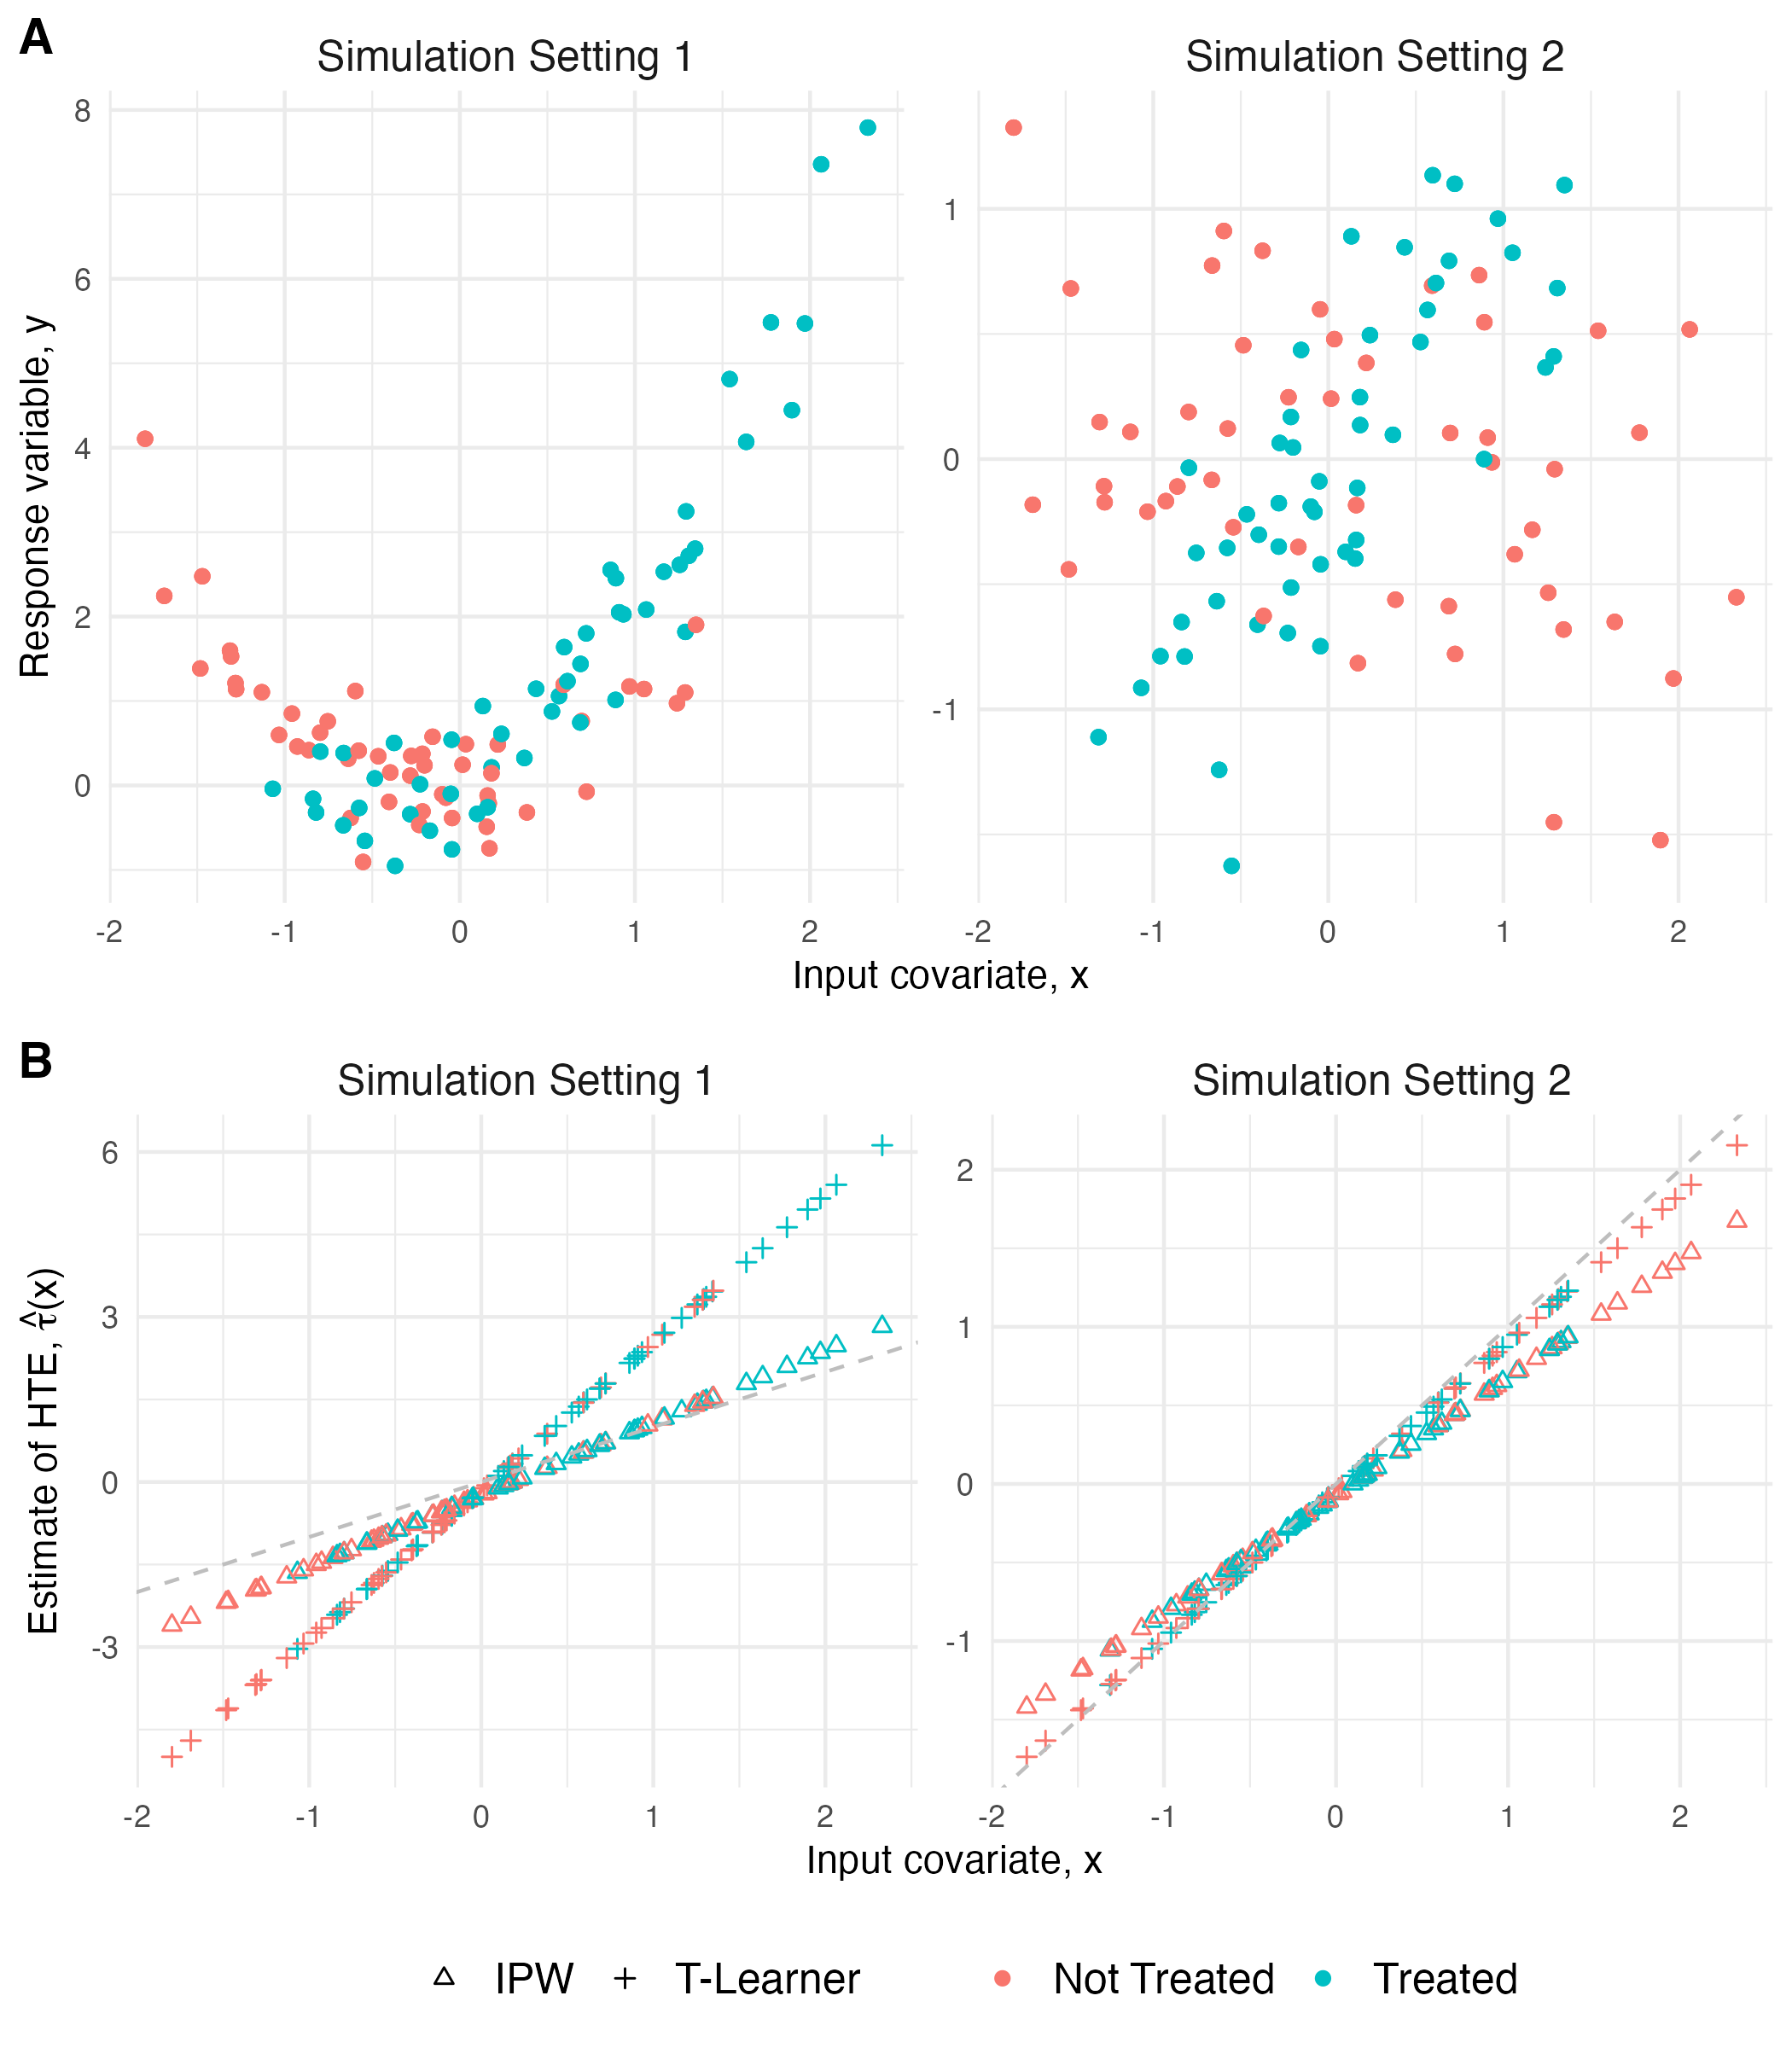
\includegraphics[width=\textwidth]{figures/chapter4/comp_figure_without_dr.png}
\caption{Simulation Settings~1~and~2 with \textbf{A}: the response variable $y$, and \textbf{B}: estimates of $\hat{\tau}(x)$ for each simulated data point according to the $T$-Learner (cross) and \gls{ipw} (triangle) strategies. The true \gls{cate}, $\tau(x)$, is shown with a grey dashed line.  \label{fig:comp_t_ipw}}
\end{figure}
Under certain conditions, the DR-Learner can be shown to produce optimal convergence rates amongst classes of models based on composition of \gls{ipw} and conditional regression functions \citep{kennedy_towards_2022}. We won't go into these conditions in detail here, but can begin to appreciate the underlying ideas by investigating the two extreme cases we've discussed. Firstly, let's assume in Step~(1) of the DR-Learner, we correctly estimate propensity (i.e. $\pihat = \pi$) but do not correctly estimate our conditional regression functions (i.e. $(\muhat_0, \muhat_1) \neq (\mu_0, \mu_1)$). We can then write that 
\begin{align*}
    \Tilde{Y}_{DR} & =  \frac{A - {\pi}(X)}{{\pi}(X)(1-{\pi}(X))}\Big( Y - \muhat_A(X)\Big) + \muhat_1(X) - \muhat_0(X) \\
    & = \frac{A - {\pi}(X)}{{\pi}(X)(1-{\pi}(X))}\Big(A\big(Y^{(1)} - \muhat_1(X)\big) + (1-A)\big(Y^{(0)} - \muhat_0(X) \big)\Big) \\
    & \hspace{50pt} + \muhat_1(X) - \muhat_0(X)
\end{align*}
and therefore that
\begin{align*}
    \bbE[\Tilde{Y}_{DR} | X=x]  & = \frac{1}{\pi(x)(1-\pi(x))} \Big(\bbE[AY^{(1)} - A\muhat_1(x) - A\pi(x)Y^{(1)} + A\pi(x)\muhat_1(x) \ - \\
    & \hspace{50pt} (1-A)\pi(x)Y^{(0)} + (1-A)\pi(x)\muhat_0(x) \ | \ X=x ] \Big) + \muhat_1(x) - \muhat_0(x) \\ 
    & = \frac{1}{\pi(x)(1-\pi(x))} \Big( \pi(x)\mu_1(x) - \pi(x)\muhat_1(x) - \pi(x)^2\mu_1(x) + \\
    & \hspace{50pt} \pi(x)^2\muhat_1(x) - (1-\pi(x))\pi(x)\mu_0(x) + (1-\pi(x))\pi(x) \muhat_0(x) \Big) + \\
    & \hspace{50pt} \muhat_1(x) - \muhat_0(x) \\
    & = \frac{1}{\pi(x)(1-\pi(x))]} \Big( \pi(x)\big(\mu_1(x) - \muhat_1(x) - \pi(x)(\mu_1(x) - \muhat_1(x)) \big) - \\
    & \hspace{50pt} \pi(x)(1-\pi(x))\big( \mu_0(x) - \muhat_0(x) \big) \Big) + \muhat_1(x) - \muhat_0(x) \\
    & = (\mu_1(x) - \muhat_1(x)) - (\mu_0(x) - \muhat_0(x)) + \muhat_1(x) - \muhat_0(x) \\ 
    &= \mu_1(x) - \mu_0(x) = \tau(x),
\end{align*}
where here in the first equality we are leveraging that $A^2 = A$ and (equivalently) that $A(1-A) = 0$, and in the second equality we make use of the fact that $Y\perp A \ | \ X$ and that $\mu_a(x) := \bbE[Y^{(a)}|X=x]$.

Secondly, let's now assume we've estimated the conditional regression functions well (so that $(\muhat_1, \muhat_0) = (\mu_1, \mu_0)$). Then we can say that 

\begin{align*}
    \bbE[\Tilde{Y}_{DR} | X = x] & = \bbE [\frac{A - \pihat(x)}{\pihat(x)(1 - \pihat(x)} \Big( A (Y^{(1)} - \mu_1(x)) + \\
    &\hspace{50pt} (1-A)(Y^{(0)} - \mu_0(x)) \Big) \ | \ X=x] \ +  \mu_1(x) - \mu_0(x)  \\
    & = \frac{1}{\pihat(x)(1-\pihat(x))} \bbE [ \Big( A(Y^{(1)} - \mu_1(x)) -\pihat(x)A(Y^{(1)} - \mu_1(x)) \ - \\
    & \hspace{50pt} \pihat(x) (1-A)(Y^{(0)} - \mu_0(x))\Big) \ | \ X=x] + \mu_1(x) - \mu_0(x) \\
    & = \frac{1}{\pihat(x)(1-\pihat(x))} \bbE [\Big( \pi(x) (\mu_1(x) - \mu_1(x)) - \\
    & \hspace{50pt} \pi(x)\pihat(x)(\mu_1(x) - \mu_1(x)) - \\
    & \hspace{50pt} (1-\pi(x))\pihat(x)(\mu_0(x) - \mu_0(x)) \Big) \ | \ X=x ] + \mu_1(x) - \mu_0(x) \\
    & = \mu_1(x) - \mu_0(x) = \tau(x),
\end{align*}
where again we've used that $A^2 = A$, $A(1-A) = 0$, the conditional independence of $A$ and $Y^{(a)}$, and the definition of the conditional regression functions $Y^{(a)}$.
Without elaborating further on the asymptotic properties of the doubly robust estimator, we can see from the above where robustness to each type of model misspecification arises. We reconsider Examples~\ref{ex:ipw_better} and~\ref{ex:t_better}, with the DR-Learner also included (Figure~\ref{fig:comp_t_ipw_dr}). While we don't see the DR-Learner perform the outright best in either scenario, we do see it lives up to its doubly robust credentials, performing well in both cases. In scenarios where both propensity and conditional regression estimates are misspecified, we cannot expect faithful prediction of treatment effect.

\begin{figure}[!tpb] 
\centering
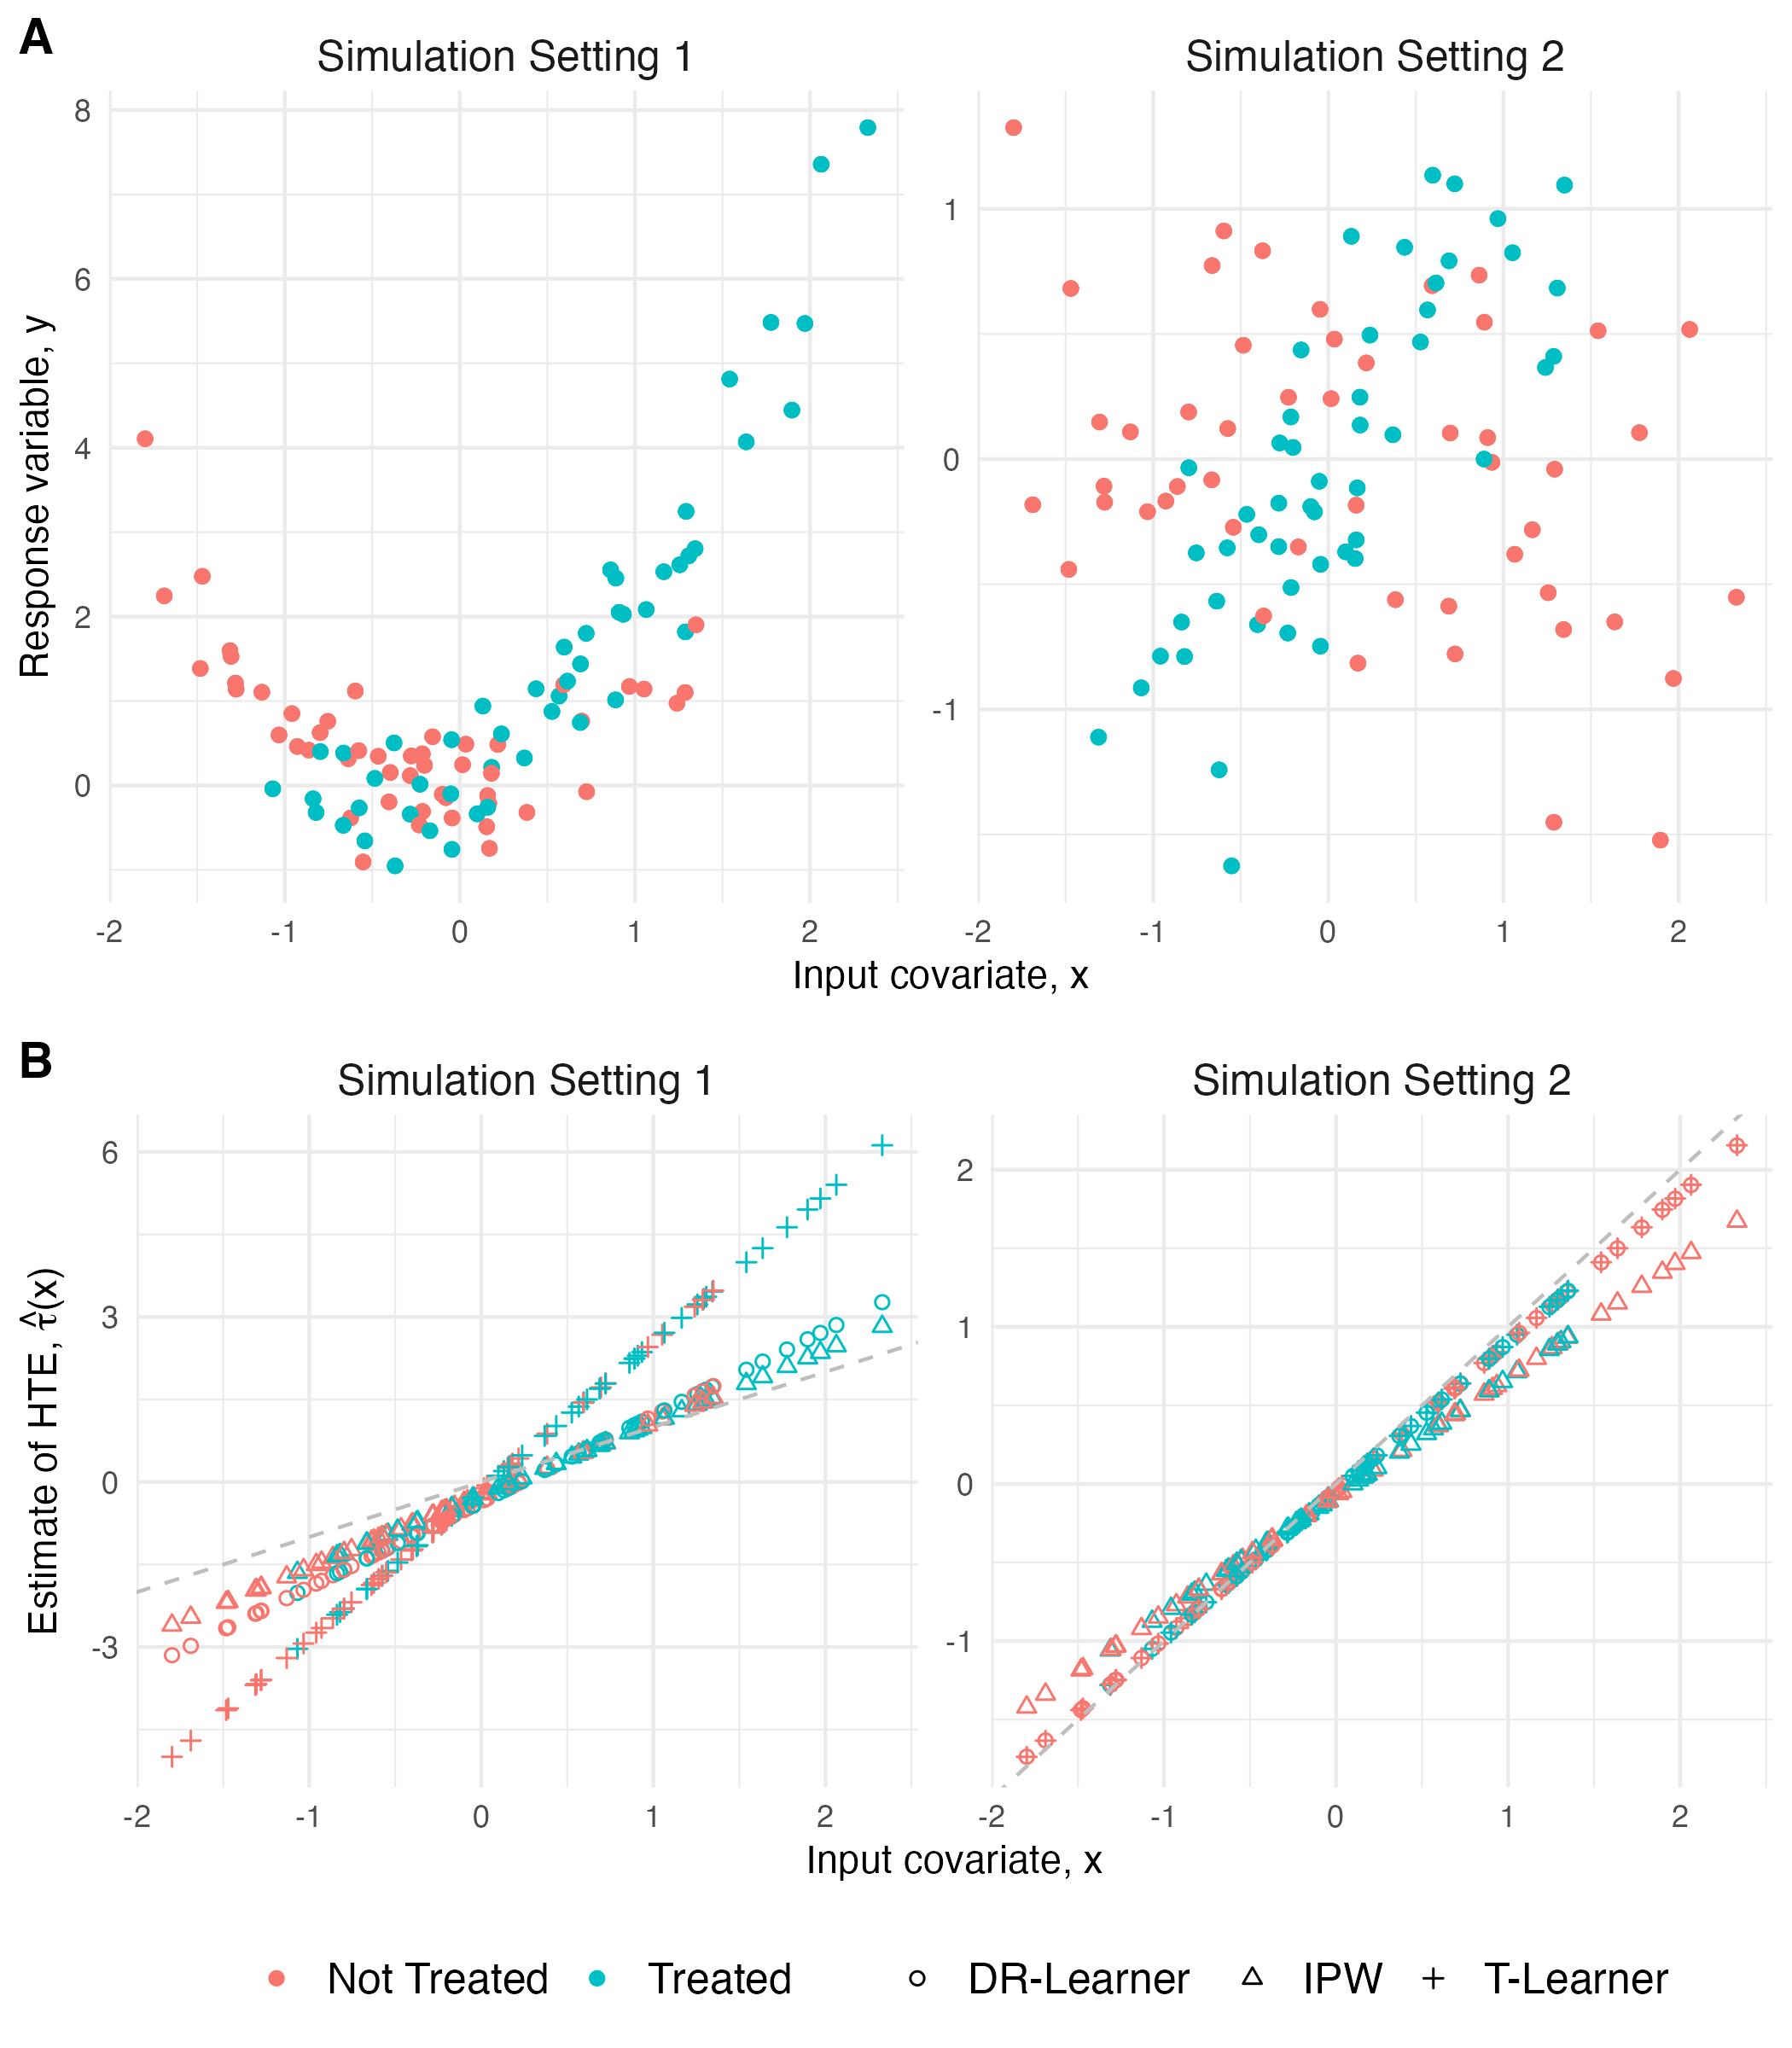
\includegraphics[width=\textwidth]{figures/chapter4/comp_figure_with_dr.png}
\caption{Simulation Settings~1~and~2 with \textbf{A}: the response variable $y$, and \textbf{B}: estimates of $\hat{\tau}(x)$ for each simulated data point according to the $T$-Learner (cross), \gls{ipw} (triangle), and DR-Learner (circle) strategies. The true \gls{cate}, $\tau(x)$, is shown with a grey dashed line.  \label{fig:comp_t_ipw_dr}}
\end{figure}


\subsection{Causal forests} \label{sec:causal_forests}

Before we describe causal forests, which were developed and implemented as a specific instance of so-called `generalised random forests' \citep{athey_generalized_2019, athey_estimating_2019}, we first describe briefly the process behind fitting (or `growing') random forests in general. Random forests were introduced by \citet{breiman_random_2001} and have been in the standard repertoire of machine learning methods ever since, noted in particular for their strong out-of-the-box performance with little parameter tuning, even when applied to high-dimensional data. Here we'll discuss only the application of random forests to regression problems, although classification forests proceed in a very similar fashion.

Random forest models are \emph{ensembles} (weighted combinations) of \emph{decision trees}. Decision trees rely on a recursive partition of the domain space (in our case $\mathcal{X}$) into rectangular subspaces known as `leaves' (see Figure~\ref{fig:recursive} for a visual example). Within each leaf, a representative value is used as the regression output, typically the mean of all training sample output values within that leaf. Branching of the tree is determined by choosing a threshold at which to subdivide the covariate space. This is often chosen so as to minimise the resultant variance of the resultant within-branch training sample outputs. The set of candidate covariates on which to threshold is chosen out of a random subset whose size is a hyperparameter of the algorithm. Other hyperparameters determine how deep and wide a decision tree is allowed to grow. Random forests, as the name suggest, average over the predictions of many trees, each trained on a randomly selected subset of the training data. For a given number of trees $B$, each tree $b$ results in a partition function $L_b \colon \mathcal{X} \rightarrow 2^{\mathcal{X}}$ which, given a point $x \in \mathcal{X}$, maps to the leaf of the tree $b$ in which resides so that $x \in L_b(x)$. A prediction for a point $x$ on a given tree $b$ is given by the weighted average
\[ \sum_{i=1}^{n} \frac{\mathbbm{1} \{X_i \in L_b(x), i \in \mathcal{S}_b\}Y_i}{|\{i \colon X_i \in L_b(x), i \in \mathcal{S}_b\}|},\]
where $\mathcal{S}_b$ is the random subsample of the training set chosen for tree $b$. We can then say that a prediction from the entire random forest for a point $x$ is given by 
\[\frac{1}{B}\sum_{b=1}^{B} \sum_{i=1}^{n} \frac{\mathbbm{1} \{X_i \in L_b(x), i \in \mathcal{S}_b\}Y_i}{|\{i \colon X_i \in L_b(x), i \in \mathcal{S}_b\}|} = \sum_{i=1}^{n} \alpha_i(x) Y_i, \]
\[ \text{where} \ \alpha_i(x) := \frac{1}{B} \sum_{b=1}^B \frac{\mathbbm{1} \{X_i \in L_b(x), i \in \mathcal{S}_b\}Y_i}{|\{i \colon X_i \in L_b(x), i \in \mathcal{S}_b\}|}.\]
\begin{figure}
    \centering
    
\includegraphics[width=\textwidth]{figures/chapter4/recursive.png}
    \caption{Example of a recursive partition of a space into `leaves' in two dimensions, reproduced from \citet{reeve_adaptive_2021}.}
    \label{fig:recursive}
\end{figure}

Causal forests, produced by an adaptation of the random forests algorithm, are inspired by the $R$-Learner approach of \citet{nie_learning_2017}. To motivate this approach we note that, under the standard causal assumptions,
\begin{align*} 
Y - \mu(X) & = Y^{(1)} + (1-A)Y^{(0)} - \pi(X)\bbE[Y^{(1)}|X] - (1-\pi(X))\bbE[Y^{(0)}|X]
\\  
& = AY^{(1)} + (1-A)Y^{(0)}- \bbE[Y^{(0)}|X] - \pi(X)\tau(X) \\
& = A(Y^{(1)} - \bbE[Y^{(1)}|X]) + (1-A)(Y^{(0)}- \bbE[Y^{(0)}|X]) + (A-\pi(X))\tau(X) \\
& = (Y - \bbE[Y|X,A]) + (A-\pi(X))\tau(X).
\end{align*}
Here the first term $(Y-\bbE[Y|X,A])$ is the intrinsic variation due to randomness in $Y$ after all controls. \citet{nie_learning_2017} therefore propose first estimating the propensity function $\pihat(x)$ and (marginal) regression function $\muhat(x)$. These are then combined into a target for optimisation, such that $\hat{\tau}$ is selected satisfying\footnote{The original authors also included a regularisation term, which we omit for simplicity.} 
\[\hat{\tau} \in \argmin_{\tau} \Big\{\frac{1}{n}\sum_{i=1}^{n} \bigg( \big(y_i - \muhat(x_i)\big) - \big(a_i - \pihat(x_i)\big)\tau(x_i)\bigg)^2  \Big\}.\]
To adapt this method to the regression forest setting, \citet{athey_generalized_2019} first fit forests for $\muhat$ and $\pihat$, and for each leaf select a constant value of $tau$ minimising the expression above for the relevant leaf/branch. To eliminate bias, at each point they replace $\muhat(x)$ and $\pihat(x)$ with their \emph{out-of-bag} estimates $\muhat^{(-i)}(x_i)$ and $\pihat^{(-i)}(x_i)$, where in the given regression forests only leaves not containing the given training sample are used for prediction\footnote{If not in the context of random forests, `out-of-bag' may equally be replaced by `out-of-fold' for cross-validated models.}.


\subsection{Regularisation} \label{sec:regularisation_hte}
Another view of the two heuristic extremes described in Section~\ref{sec:doublerobustness} is as a balance between  `information sharing' across the estimated conditional regression functions $\muhat_0$ and $\muhat_1$, and allowing them to be as flexible as possible in order to capture nuances to the difference between them (i.e. the treatment effect). \citet{shalit_estimating_2017} proposed a method based on representation learning, in which three functions are learned: $\Phi(x), m_0(x), m_1(x)$, such that $\muhat_a(x) := m_a(\Phi(x))$. In this way information is shared between $\muhat_0$ and $\muhat_1$ via the embedding $\Phi$. The strength of this sharing is determining by applying a regularisation term to the loss function when fitting all three functions simultaneously, which penalises distributional divergence between $\Phi(X) \ | \ A = 1$ and $\Phi(X)  \ | \ A = 0$. 

We let $\tau_{\Phi, m_0, m_1}(x) := m_1(\Phi(x)) - m_0(\Phi(x))$ to refer to the estimate of \gls{cate} derived from these functions. Here we measure the success of this estimate with expected \emph{precision in estimation heterogeneous treatment effect}, as defined in \citet{hill_bayesian_2011} and used in \citet{shalit_estimating_2017}.
\[
\epsilon_{PEHE}(\Phi, m_0, m_1) :=  \int_{\mathcal{X}} \big(\hat{\tau}_{\Phi, m_0, m_1}(x) - \tau(x) \big)^2p(x) dx, 
\]
where $p(x)$ is the density of the variable $X$ over its domain $\mathcal{X}$. Here we assume that $\Phi \colon \mathcal{X} \rightarrow \mathcal{R}$ is a one-to-one twice differentiable function with image $\mathcal{R}$ and inverse $\Phi \colon \mathcal{R} \rightarrow \mathcal{X}$. We define $p_{\Phi}^{A=a}(r) := p_{\Phi}(r|A=a)$ to be the conditional density of the image $R = \Phi(X)$ under treatment $A=a$. 

As mentioned above, our strategy will be to regularise the distributional distance between the distributions $R | A = 1$ and $R | A =0$. To do so, we will need an appropriate distance measure. For this, we employ the \gls{ipm} family. These are defined for two density functions $p$, $q$ over the domain $\mathcal{R}$. For a family $G$ of functions $g \colon \mathcal{R} \rightarrow \mathbb{R}$, we define 

\[ \mathrm{IPM}_G(p,q) := \sup_{g \in G} \Big| \int_{\mathcal{R}} g(s)\big(p(s)-q(s)\big)ds\Big|.\]
The \gls{ipm} metrics include, for an appropriate choice of function family $G$, the maximum mean discrepancy \citep{gretton_covariate_2008} and the Wasserstein distance \citep{villani_optimal_2009, sriperumbudur_empirical_2012, cuturi_sinkhorn_2013}. The aim of regularising the distributional distance between the distributions of our two conditional representations is to bound the divergence betwwen `factual' and `counterfactual' loss. To do so, we let $L \colon \mathcal{Y} \times \mathcal{Y} \rightarrow \mathbb{R}$ be a loss function and $\ell_{\Phi, m_0, m_1} \colon \mathcal{X} \times \{0,1\} \rightarrow \mathbb{R}$ be the expected loss at the point $(x,a)$, i.e. $\ell_{\Phi, m_0, m_1} := \int_\mathcal{Y} L(y^{(a)}, m_a(\Phi(x)))p(y^{(a)}|X=x)dy^{(a)}$. We then define factual and counterfactual losses $\epsilon_F(\Phi, m_0, m_1)$ and $\epsilon_{CF}(\Phi, m_0, m_1)$ respectively via
\begin{align*}
    \epsilon^{a=1}_F(\Phi, m_0, m_1) & := \int_{\mathcal{X}} \ell_{\Phi, m_0, m_1}(x, 1)p^{a=1}(x)dx, \\
    \epsilon^{a=0}_F(\Phi, m_0, m_1) & := \int_{\mathcal{X}} \ell_{\Phi, m_0, m_1}(x, 0)p^{a=0}(x)dx, \\
    \epsilon^{a=1}_{CF}(\Phi, m_0, m_1) & := \int_{\mathcal{X}} \ell_{\Phi, m_0, m_1}(x, 0)p^{a=1}(x)dx, \\
    \epsilon^{a=0}_{CF}(\Phi, m_0, m_1) & := \int_{\mathcal{X}} \ell_{\Phi, m_0, m_1}(x, 1)p^{a=0}(x)dx, \\
    \epsilon_F(\Phi, m_0, m_1) & := u \epsilon^{a=1}_{F}(\Phi, m_0, m_1)  + (1-u) \epsilon^{a=0}_{F}(\Phi, m_0, m_1), \\
    \epsilon_{CF}(\Phi, m_0, m_1) & := (1-u) \epsilon^{a=1}_{CF}(\Phi, m_0, m_1)  + u \epsilon^{a=0}_{CF}(\Phi, m_0, m_1), 
\end{align*}
where $u := \mathbb{P}(A=1)$. \citet{shalit_estimating_2017} prove that under certain conditions on the likelihood $\ell_{\Phi, m_0, m_1}$ and the function family $G$, there exists a constant $B_\Phi$ such that the counterfactual and factual losses defined above can be related via

\begin{align*}
    \epsilon_{CF}(\Phi, m_0, m_1)  & \leq (1-u)\epsilon_F^{a=1}(\Phi, m_0, m_1) + u\epsilon_F^{a=0}(\Phi, m_0, m_1) \\
& \hspace{50pt} + B_\Phi \mathrm{IPM}_G(p_{\Phi}^{a=1}, p_{\Phi}^{a=0}).
\end{align*} 

Their proof relies on $\Phi$ having a well-defined inverse $\Psi$, although in practice this is not always chosen to be the case. The key result here is that we have now bounded the counterfactual loss (by definition unobserved) with quantities that can be directly estimated from observed data; namely, the estimated average loss on treated patients, the estimated average loss on untreated patients, and the observed distributional distance between the two conditional representations. As a direct consequence of this, \citet{shalit_estimating_2017} are able to show that 
\[ \epsilon_{PEHE}(\Phi, m_0, m_1) \leq 2\Big(\epsilon_{F}^{a=1}(\Phi, m_0, m_1) + \epsilon^{a=0}_F(\Phi, m_0, m_1) + B_{\Phi}\mathrm{IPM}_G\big(p_\Phi^{a=1}, p_\Phi^{a=0}\big) - K\Big),\]
where $K$ does not depend on the choices of functions $\Phi, m_0, m_1$. They therefore propose empirically minimising the objective

\[\frac{1}{n}\sum_{i=1}^n w_i L(m_{a_i}(\Phi(x_i)), y_i) + \alpha \mathrm{IPM}_G\big(\{\Phi(x_i)\}_{i:a_i=0}, \{\Phi(x_i)\}_{i:a_i=1}\big),\]
\[ \text{where } w_i = \frac{a_i}{2u} + \frac{1-a_i}{2(1-u)}, u = \frac{1}{n}\sum_{i=1}^{n}a_i.\]
Here $\alpha$ is now a tunable parameter to be optimised by (for example) cross-validation.


\section{Heterogeneous treatment effects applied to survival analysis \label{sec:hte_survival}}
Having summarised several approaches and concepts for \gls{hte} estimation, we now turn to two specific (and very different) examples from recent literature on adapting estimation methods to the prediction of discrepancies in survival. These follow on from the last two examples from the previous section, namely causal forest and neural network-based distributional regularisation. As well as using different underlying methodologies, they produce starkly different outputs. Causal survival forests, like causal forests in general, learn only the target function $\hat{\tau}$, whereas the regularisation approach learns two distinct stochastic functions for survival outcomes. Notably, neither are based on a parametric statistical model for survival such as proportional hazards or accelerated failure time.

\subsection{Forests again \label{sec:surv_hte_forests}}
\citet{cui_estimating_2022} propose \glspl{csf} for \gls{hte} estimation in the presence of censored data. Based on causal forests an implemented via the same R package \texttt{grf} \citep{tibshirani_grf_2023}, their first major contribution is to propose a weighting scheme similar to the \gls{ipw} approach introduced in Section~\ref{sec:metalearners}. They then proceed to describe a correction for double robustness under misspecification of the learned censoring function. This corrective term is too technically verbose to describe in full here, so having introduced the concept of double robustness at length in Section~\ref{sec:doublerobustness} we limit ourselves here to an outline of what is achieved by this correction.

Firstly, we note that in most medical (or indeed any other) survival analyses, some maximum time horizon for uncensored data is often present. For example, in a clinical study spanning ten years, any time points greater than ten years must be censored. We may not, then, expect to be able to recover any meaningful treatment effect for this range of values. \citet{cui_estimating_2022} therefore introduce a \emph{time horizon} $h$, a deterministic transformation $\gamma$, and attempt to estimate an altered \gls{hte} funtion
\[\tau^{\gamma, h}(x) := \bbE[\gamma(T^{(1)}, h) - \gamma(T^{(0)}, h) | x = x].\]
Here the transformation $\gamma$ is restricted to satisfy $\gamma(t, h) \geq \gamma(h, h)$ for all $t \geq h>0$. The choice of the function $\gamma$ induces variations in the effect being measured, with $\gamma(t,h) = \min\{t,h\}$ inducing estimation of difference in \gls{rmst} and $\gamma(t,h) = \mathbbm{1}\{t \geq h \}$ inducing estimation of differences in survival probability. In our later analyses we investigate the application of \glspl{csf} to estimation heterogeneous effects on survival probabilities after one and two years.

In its simplest form the method of \citet{cui_estimating_2022} draws inspiration from \gls{ipcw}, the core tenet of which is to first estimate the \emph{censoring function} 
\[S_a^C(s|x) = \mathbb{P}(C \geq s | A = a, X = x).\]
We refer to this estimate as $\hat{s}_a(t|x)$. We may do this using only censored data. We could then fit a causal forest for $\gamma(T, h)$. In the language introduced in Section~\ref{sec:causal_forests}, we could express this forest as a weighted sample-wise sum with weightings 
\[\alpha_i(x)  = \frac{1}{B}\sum_{b=1}^B\frac{\mathbbm{1}\{X_i \in L_b(x), i \in \mathcal{S}_b\}}{|\{i: X_i \in L_b(x), i \in \mathcal{S}_b\}|}\}.\]
We may then simply replace this weighting $\alpha_i(x)$ with $\alpha_i(x)/ \hat{s}_{A_i}(\gamma(T_i, h) | X_i)$. This has the effect of up-weighting observations which were observed but which were unlikely to have been observed, and has been shown empirically to be broadly successful in eliminating censoring bias \citep{van_der_laan_unified_2003}.

While the \gls{ipcw} strategy may be a good baseline, it suffers from two key drawbacks: firstly, each of its censoring and treatment functions can only be learned on a subset of the available training data. Secondly, it is vulnerable to misspecification/poor fit of the censoring function $\hat{s}_a(t|x$). The solution proposed by \citet{cui_estimating_2022} entails the joint estimation of several more `nuisance' functions detailing different aspects of the censoring distribution. Taken together these are shown to provide double robustness -- an analogue to the double robustness demonstrated in Section~\ref{sec:doublerobustness}, taken here to mean robustness to either misspecification of the censoring function or misspecification of the propensity function.


\subsection{Regularisation again \label{sec:surv_reg}}
Our second example of a modern strategy for enabling survival \gls{hte} estimation returns to the distributional regularisation method proposed by \citet{shalit_estimating_2017} and discussed in Section~\ref{sec:regularisation_hte}. \citet{chapfuwa_enabling_2021} proposed an extension, \gls{csa}\footnote{They also provide a further extension, CSA-INFO, to deal with informative censoring; we omit this for simplicity.}, applicable to survival data that retains the same overall structure: learning a representation $\Phi \colon \mathcal{X} \rightarrow \mathcal{R}$ of input data $X$ taking values in $\mathcal{X}$ that serves to `share information' between two conditional regression functions defined by compositions of the representation function $\Phi$ with treatment-specific functions $m_0,m_1$. The same regularisation term, based on \glsfirst{ipm} families which include the Wasserstein distance, is used to force the learned representations $R=\Phi(X)$ to be distributionally similar regardless of the assigned treatment. 

The required extension to survival analysis is provided by replacing the deterministic functions $m_0, m_1$ with flexible regression functions (in this case provided by neural networks) dependent on a separate random input $\varepsilon$. This allows for a non-parametric specification of the distribution of survival times, as described in Section~\ref{sec:nonparametric}. Again as described in the previous section, the adapted survival loss from \citet{chapfuwa_adversarial_2018}. We therefore arrive at a strategy defined by minimising the objective 
\[\frac{1}{n}\sum_{i=1}^n w_i L(m_{a_i}(\Phi(x_i), \varepsilon), y_i, \delta_i) + \alpha \mathrm{IPM}_G\big(\{\Phi(x_i)\}_{i:a_i=0}, \{\Phi(x_i)\}_{i:a_i=1}\big),\]
\[\text{with } L(t, y, \delta) := \delta|y-t| + (1-\delta)\max\{0, y-t\} \]
and $w_i, u$ defined as in Section~\ref{sec:regularisation_hte}. In the experiments presented in later sections, we use an adapted PyTorch \citep{paszke_pytorch_2019} implementation of these metods provided by \citep{chapfuwa_enabling_2021}.

\section{Application to a combined immunotherapy dataset \label{sec:immuno_hte}}

\subsection{Data sources}

We compare two datasets comprising mutation and clinical data derived from late stage cancer patients. The first dataset, produced by \citet{zehir_mutational_2017}, is derived from a large cohort treated at \gls{mskcc}. It was produced in order to inform decisions around experimental treatment regimes for patients whose tumours had been refractory to standard care. The second, produced by \citet{hellmann_genomic_2018}, describes a smaller (but still substantial) cohort of patients at similar disease stages who were then treated with \gls{icb}. While there are differences between the two datasets in both the availability of clinical data and the specifics of patient trajectory, the two studies provide usefully comparable data sources for patients that were and were not treated by immunotherapy. Crucially, since both analyses were performed using the MSK-IMPACT targeted sequencing panel, their mutation profiling is very comparable. We describe further characteristics of each dataset below. 

\subsubsection*{Zehir et al.}
This study by \gls{mskcc} provides somatic mutation data, as well as some clinical covariates, for over 10,000 patients with late stage cancer of a variety of types. These patients were, by entry criteria, those who would be eligible to participate in clinical trials for experimental drugs. After the sequencing study was conducted, a minority (11\%; 527 patients) did indeed go on to be matched to further trials on the basis of their mutation profile. Overall survival statistics are provided relative to a baseline given by the time point at which the procedure for recovering the sequencing sample was performed. Many samples were taken from metastatic sites, and some patients had multiple samples recovered. The fact that all tumours sequenced in the study were those of late stage cancers is emphasised by the authors as allowing a fuller picture of the mutations associated with cancer development and response to first-line treatment. Clinical features available include detailed cancer type information, metastatic status, sex, and smoking history.

\subsubsection*{Hellman et al.}
This dataset describes advanced cancer patients who did receive \gls{icb} treatment based on inhibition of \gls{pdl1}, \gls{ctla4}, or both. For these patients, overall survival was measured from the date of first \gls{icb} treatment. Clinical features available include sex, age, and drug type.

\subsection{Validating TMB}
We begin by investigating the extent to which the methods we've described for \gls{hte} estimation can recapitulate the known relationship between \gls{tmb} and benefit from immunotherapy. This is a valuable benchmark for any modelling approach, because basing predictions on \gls{tmb} alone (alongside any available general clinical features) means working with an input of low dimension, which should present a smalelr challenge to any estimation method.

We begin by applying the causal survival forests method of \citet{cui_estimating_2022}. To restrict the focus of this demonstrative application, we consider only \gls{nsclc} patients from each of the datasets described above. To simplify matters further, we consider only patients without missing data for time-to-event, censoring status, sex, or \gls{tmb} values, and where multiple samples are available for a given patient we take only the sample with the highest sequencing coverage. After these restrictions we are left with samples from 129 immunotherapy-treated patients, and 603 not treated with immunotherapy. We take 75\% of these samples (96 immunotherapy, 452 non-immunotherapy) as a training dataset. We apply causal survival forests to predict differences in probability of survival after one and two years, as described in Section~\ref{sec:surv_hte_forests}.

We present out-of-bag predictions of difference in survival probability for survival after one and two years for each patient in the training set using this method in Figure~\ref{fig:immuno_train_samples_hte_predictions}. For two year survival we see a substantial improvement in expected benefit from immunotherapy, with increased \gls{tmb} at low \gls{bmr}, before a plateau at around 20mut/Mb. Sex, the only clinical covariate available across both datasets (more on this later), appears to play a role fairly independently from \gls{tmb}. Within this trend, male patients appear to be consistently benefiting more from immunotherapy across \gls{tmb} values.

\begin{figure}[!tpb] 
\centering
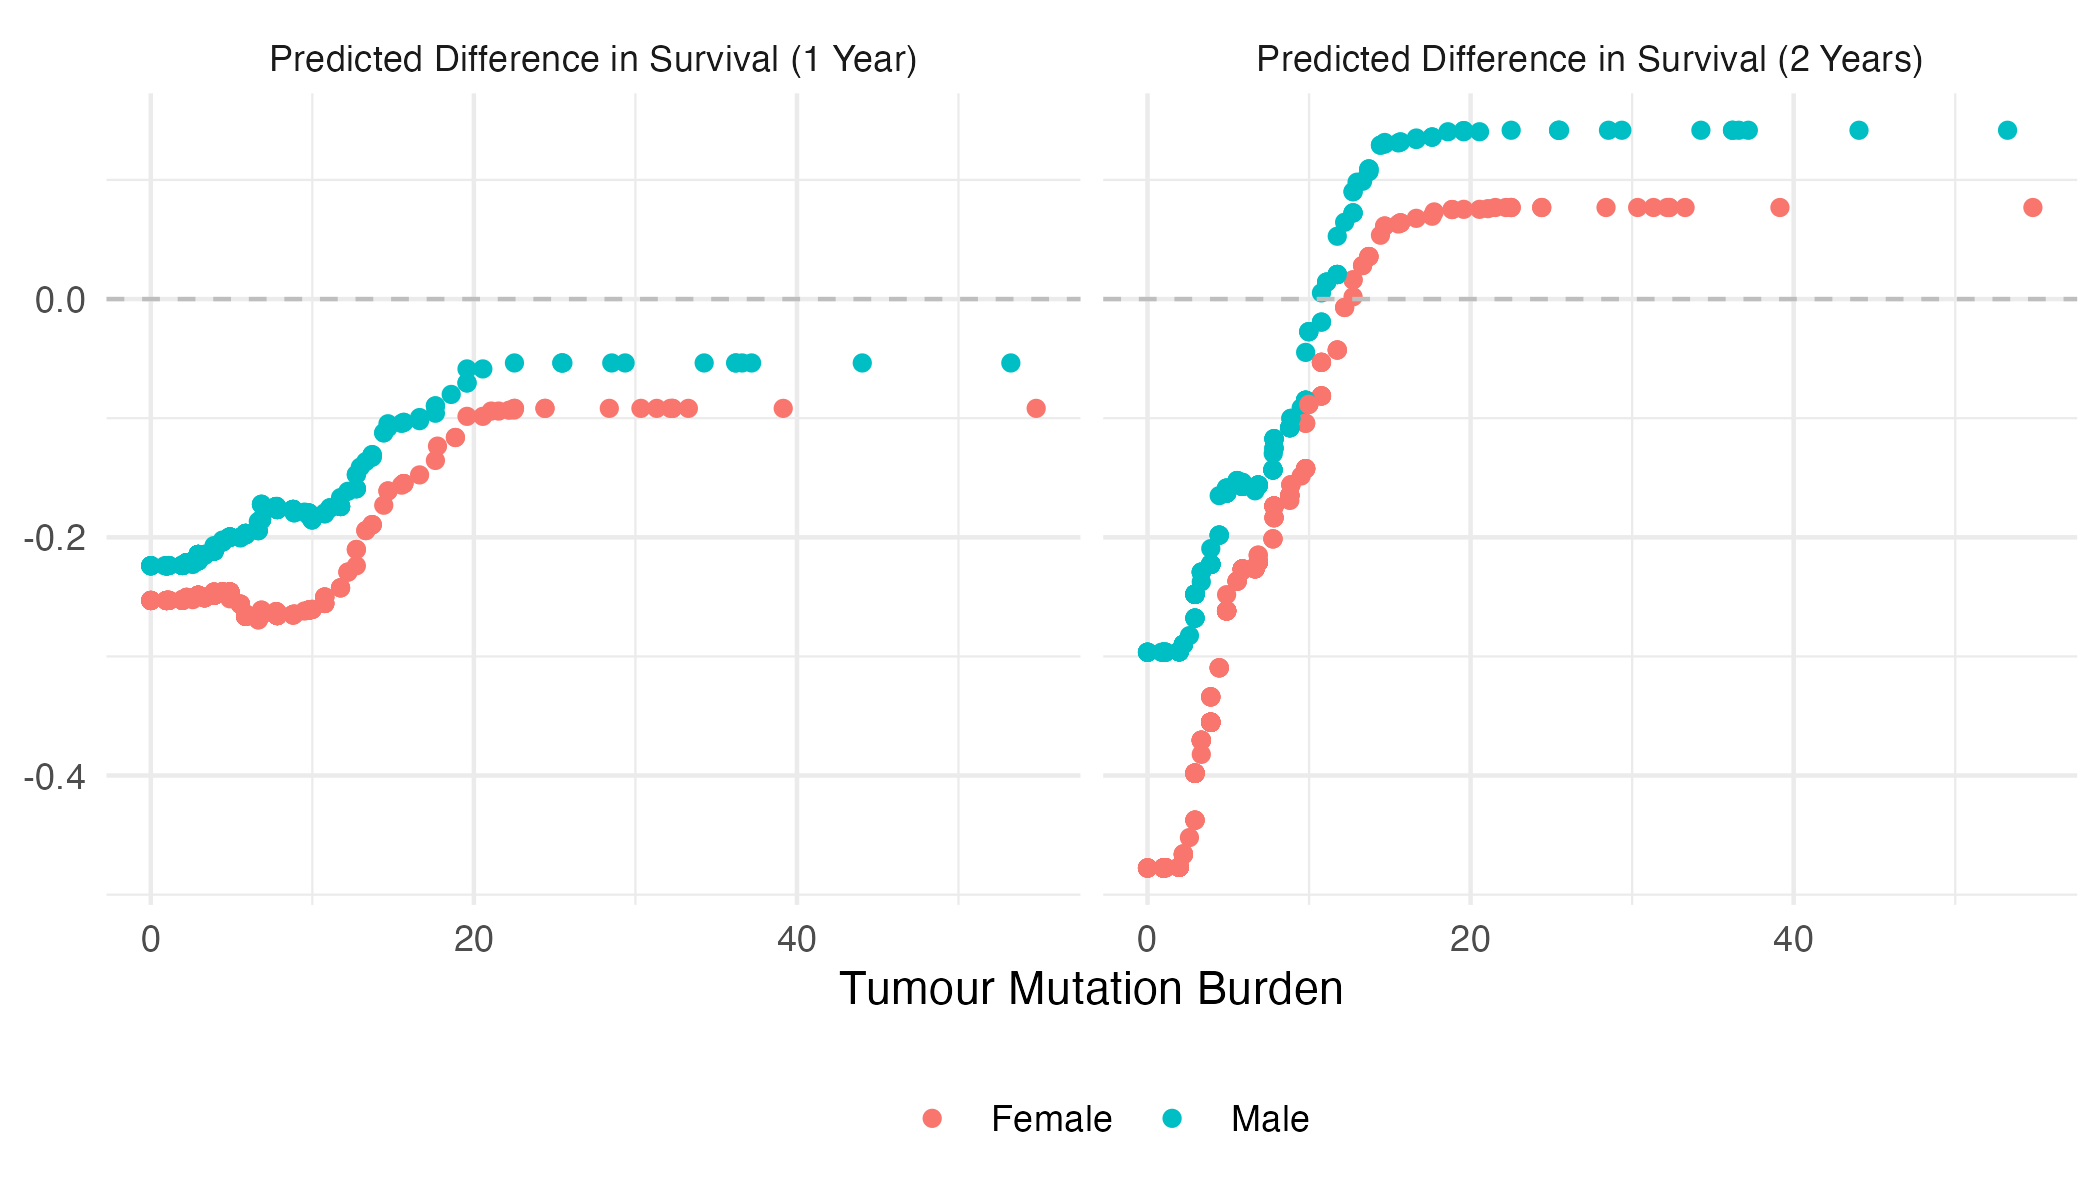
\includegraphics[width=\textwidth]{figures/chapter4/immuno_train_samples_hte_predictions.png} 

\caption{Out-of-bag CSF predictions of difference of probability of 1- and 2-year survival (left and right panels respectively) after treatment with immunotherapy for non-small cell lung cancer patients.  \label{fig:immuno_train_samples_hte_predictions}}
\end{figure}


Interestingly, while a strong dependence on \gls{tmb} is observed, the highest level of estimated benefit from immunotherapy is fairly low, and indeed for the majority of patients with low \gls{tmb} we estimate negative benefit from immunotherapy treatment. We hypothesise that this is due to uncaptured differences in typical clinical features between the two datasets. As mentioned above, to perform this analysis we were only able to utilise clinical factors that were recorded across both studies. As a conglomeration of multiple studies itself, the \citet{zehir_mutational_2017} dataset in particular did not make available several pieces of data that would be expected to impact disease trajectories significantly. The two most important of these, which would certainly be necessary to strengthen any associations learned here, would be patient age, and disease stage. Systematic variation in either would be likely to impact the difference in average rate of two-year survival between the two data sources and skew overall estimation of immunotherapy benefit (even if the relationship with \gls{tmb} was accurately captured). This same trajectory is observed for one-year survival but the lack of overall ascribed benefit to immunotherapy is even clearer; in this case for no values of \gls{tmb} does the inferred survival benefit exceed net neutrality. The overall variation in benefit with increased \gls{tmb} is also lower, despite the similar shape of the inferred response curve. It is not clear why the overall (presumed) underestimate of benefit from immunotherapy is so much more pronounced after twelve months than twenty four. It has been noted that \gls{icb}-type immunotherapy can particularly effective at producing long-term survival benefits to the subset of patients who receive some benefit \citep{putzu_duration_2023}. This, if the case here, may explain to some degree this qualitative difference. 

We also fitted neural network-based conditional regression functions as described in Section~\ref{sec:surv_reg}. This was done performed using a neural network with a single hidden layer of dimension 10 and an output also of dimension 10 for $\Phi(x)$. The functions $m_0,m_1$ were also neural networks with a single hidden layer of dimension 10. The random input $\varepsilon$ was of size ten, with each element independently distributed according to $U[0,1]$. We performed selection of the regularisation parameter $\alpha$ by likelihood minimisation on the validation set across the range $\alpha \in \{10^{-1}, 10^{0}, 10^1, 10^2, 10^3\}$. We report the output of these runs in Figure~\ref{fig:alpha_selection}, and selected $\alpha = 10^1$. We then used this fitted model to sample 200 estimated survival times under each treatment for covariates corresponding to each patient in the training set, and from these calculated the estimated differences in survival probability after one and two years (as for the causal forests example above). These predictions are given in Figure~\ref{fig:immuno_train_samples_nn_hte_predictions}.

\begin{figure}[!tpb] 
\centering
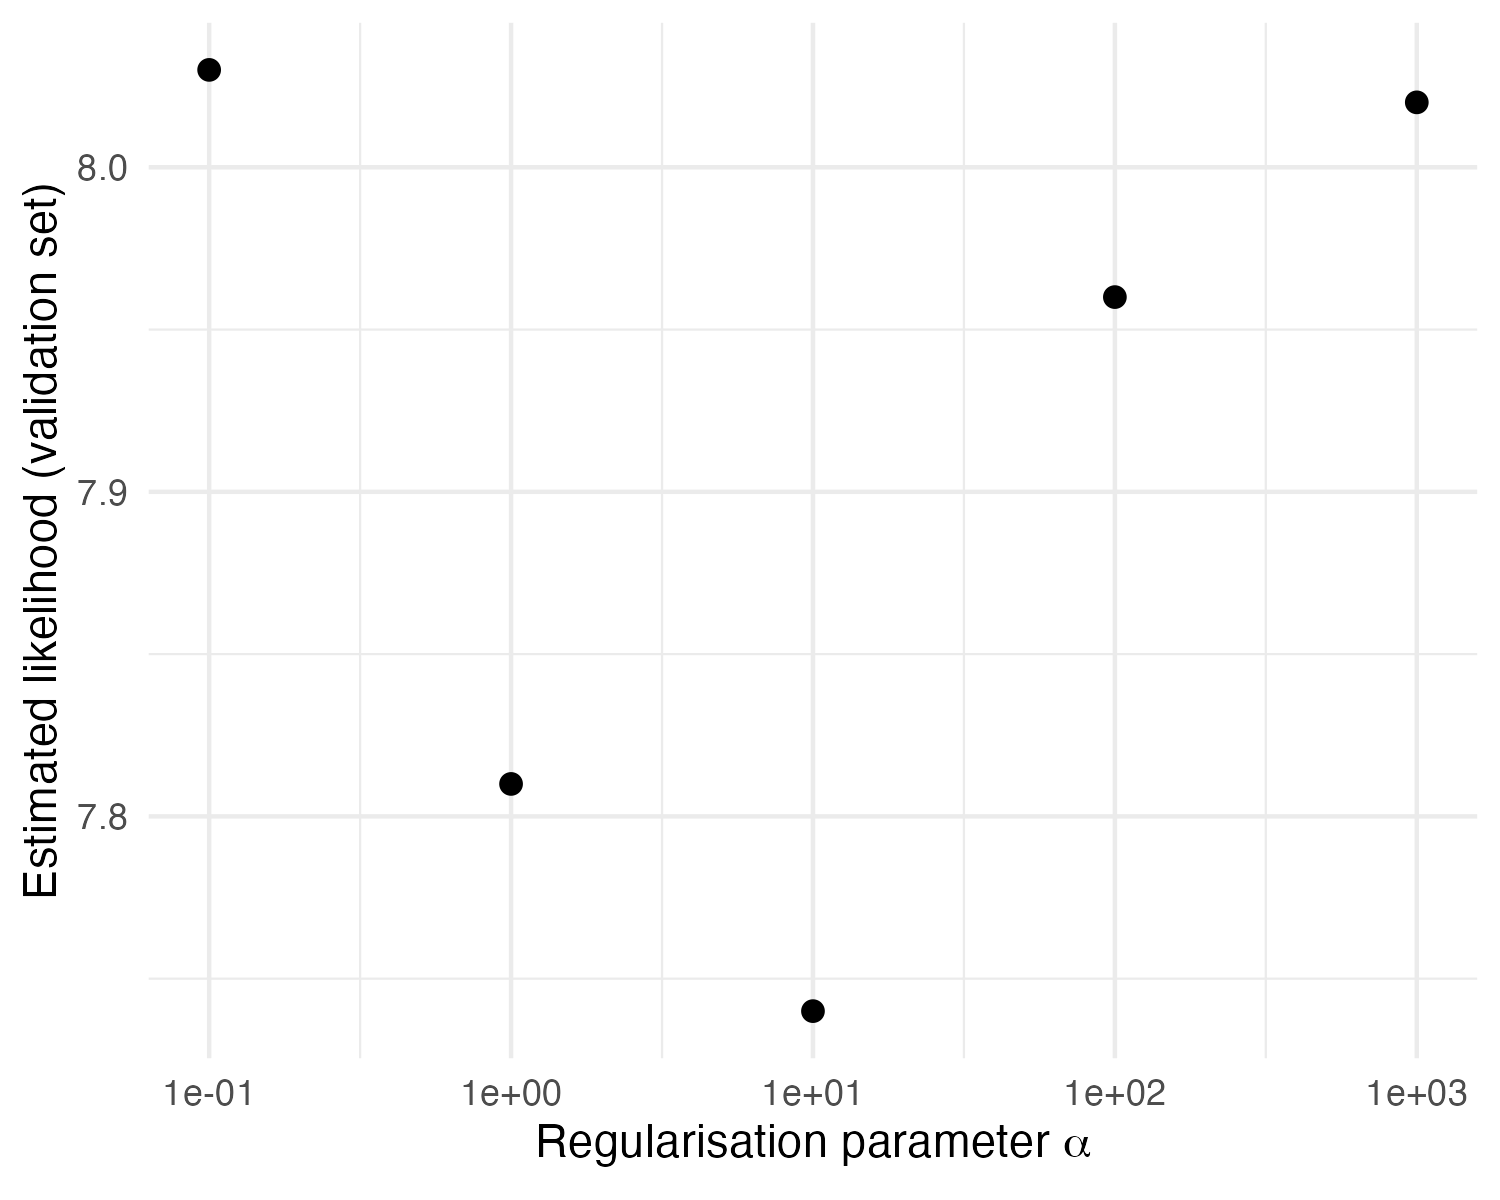
\includegraphics[width=.6\textwidth]{figures/chapter4/alpha_selection_fig.png} 

\caption{Selection of $\alpha$ penalisation parameter for CSA model. A value of $\alpha=10^1$ was selected. \label{fig:alpha_selection}}
\end{figure}

\begin{figure}[!tpb] 
\centering
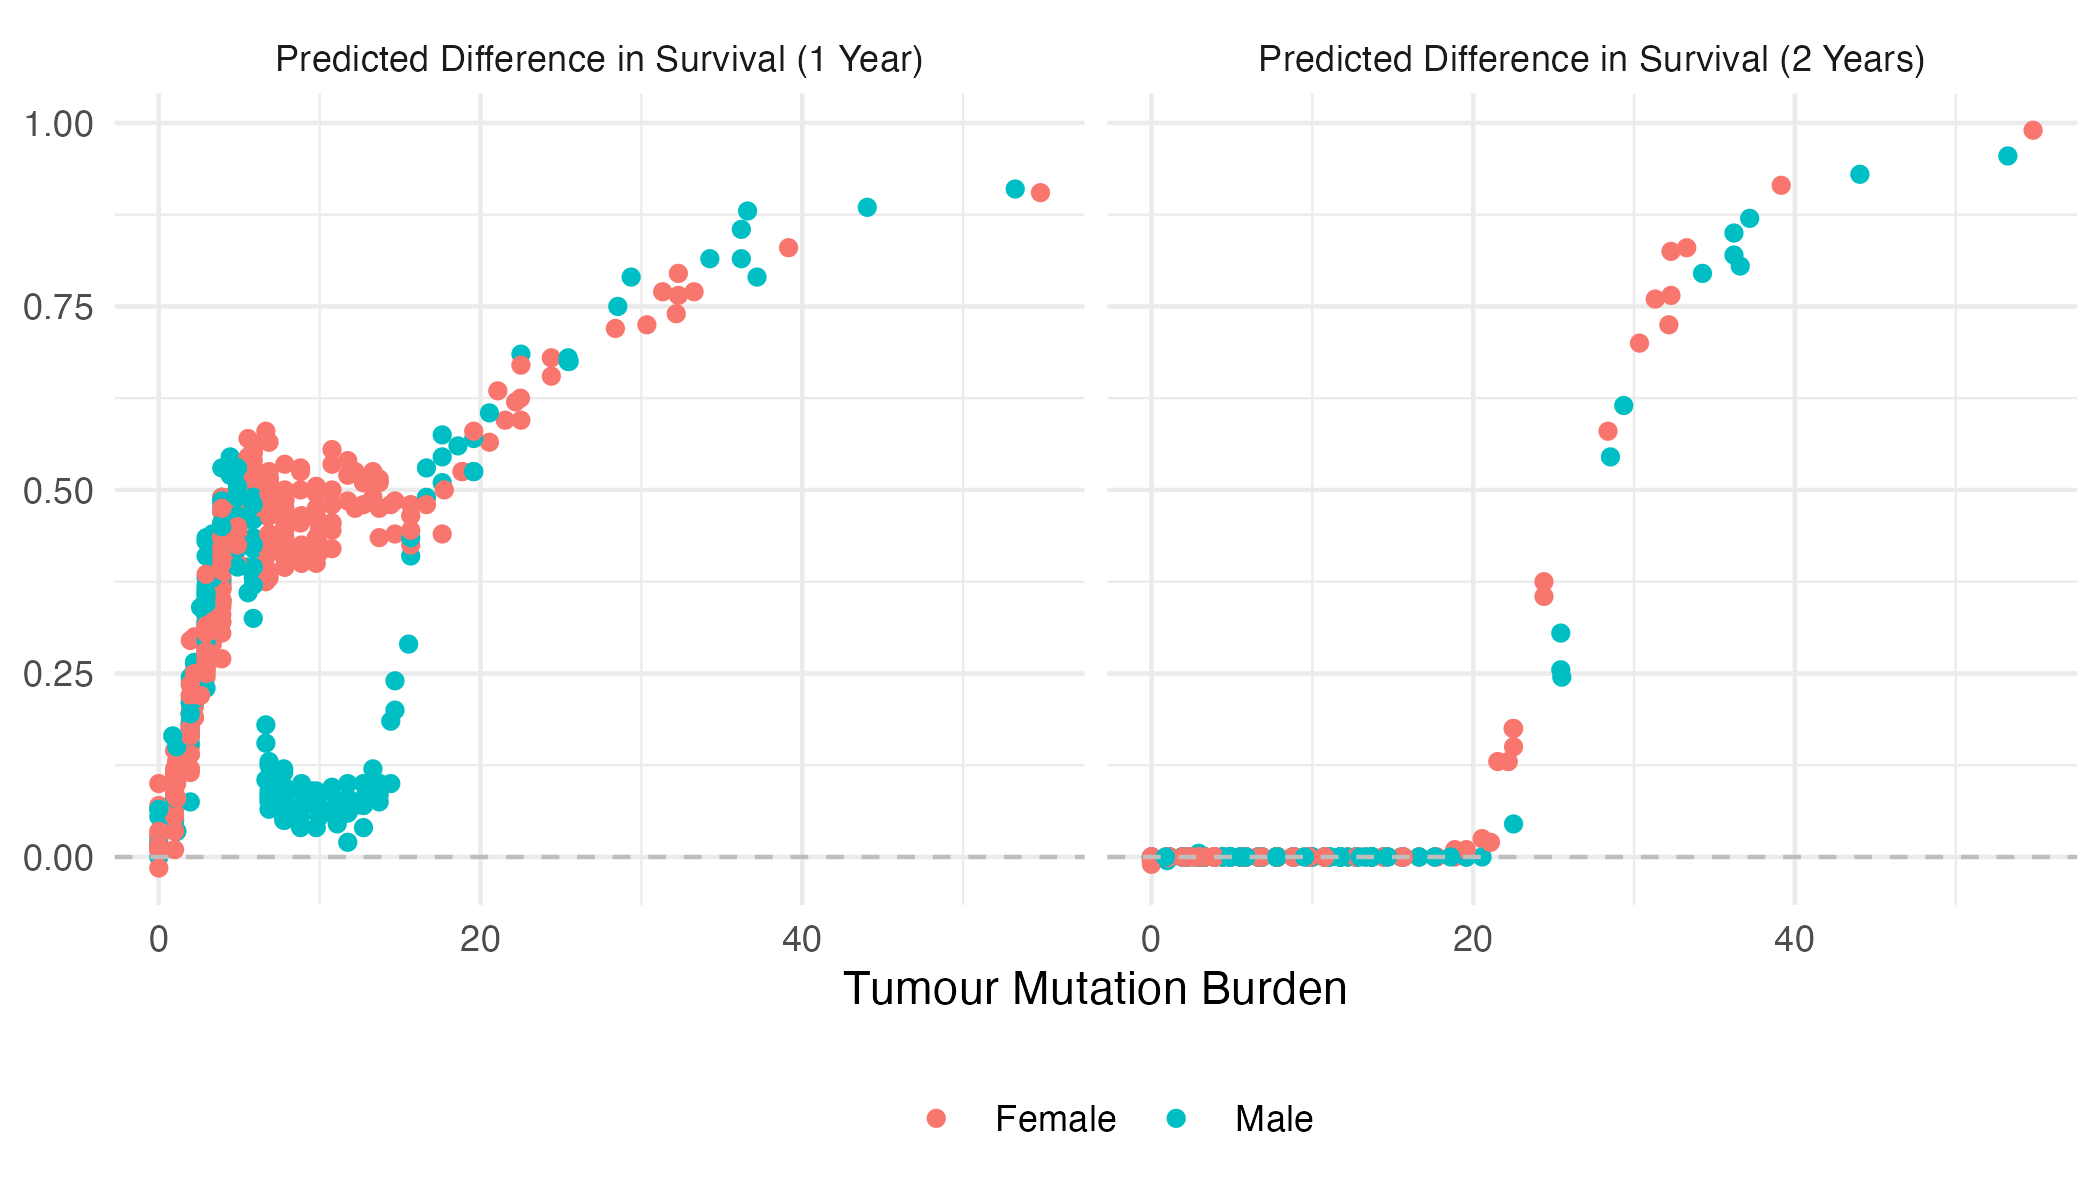
\includegraphics[width=\textwidth]{figures/chapter4/train_samples_nn_predictions.png} 

\caption{CSA neural network predictions of difference of probability of 1- and 2-year survival (left and right panels respectively) after treatment with immunotherapy for non-small cell lung cancer patients. \label{fig:immuno_train_samples_nn_hte_predictions}}
\end{figure}

Firstly, we see a clearly similar overall picture of response to increased \gls{tmb} in estimated treatment benefit as in the previous analysis. In both cases benefit rises with \gls{tmb}, with a plateau after around 20mut/MB in the case of one-year survival. Strikingly, the predicted range of benefit is much higher than in the causal forests analysis; here for both one- and two-year survival there are very few samples with a predicted negative treatment effect. This may well be principally driven by more pessimistic predictions of overall survival time. Particularly in the two-year survival case, many input data points are assigned zero probability of survival beyond two years under either treatment regime. This is difficult to compare directly with causal survival forests, since the latter method does not provide predictions of survival, instead providing simply an prediction of the difference in survival probabilities.




\subsection{Exploring more general markers}
In order to explore signatures of response depending on more than just on clinical factors and \gls{tmb}, we include nonsynonymous mutation counts for each gene in the MSK-IMPACT gene panel. This panel consists (unsurprisingly) of 341 gene targets. Some samples in the given datasets were profiled with more extensive gene panels, so we restricted our analysis only to the genes covered by all panels. We fitted causal survival forests based on these mutation counts, patient sex, and \gls{tmb}. We then computed variable importance measures for each covariate, with all non-zero values shown in Figure~\ref{fig:immuno_panel_variable_importance}. 

\begin{figure}[!tpb] 
\centering
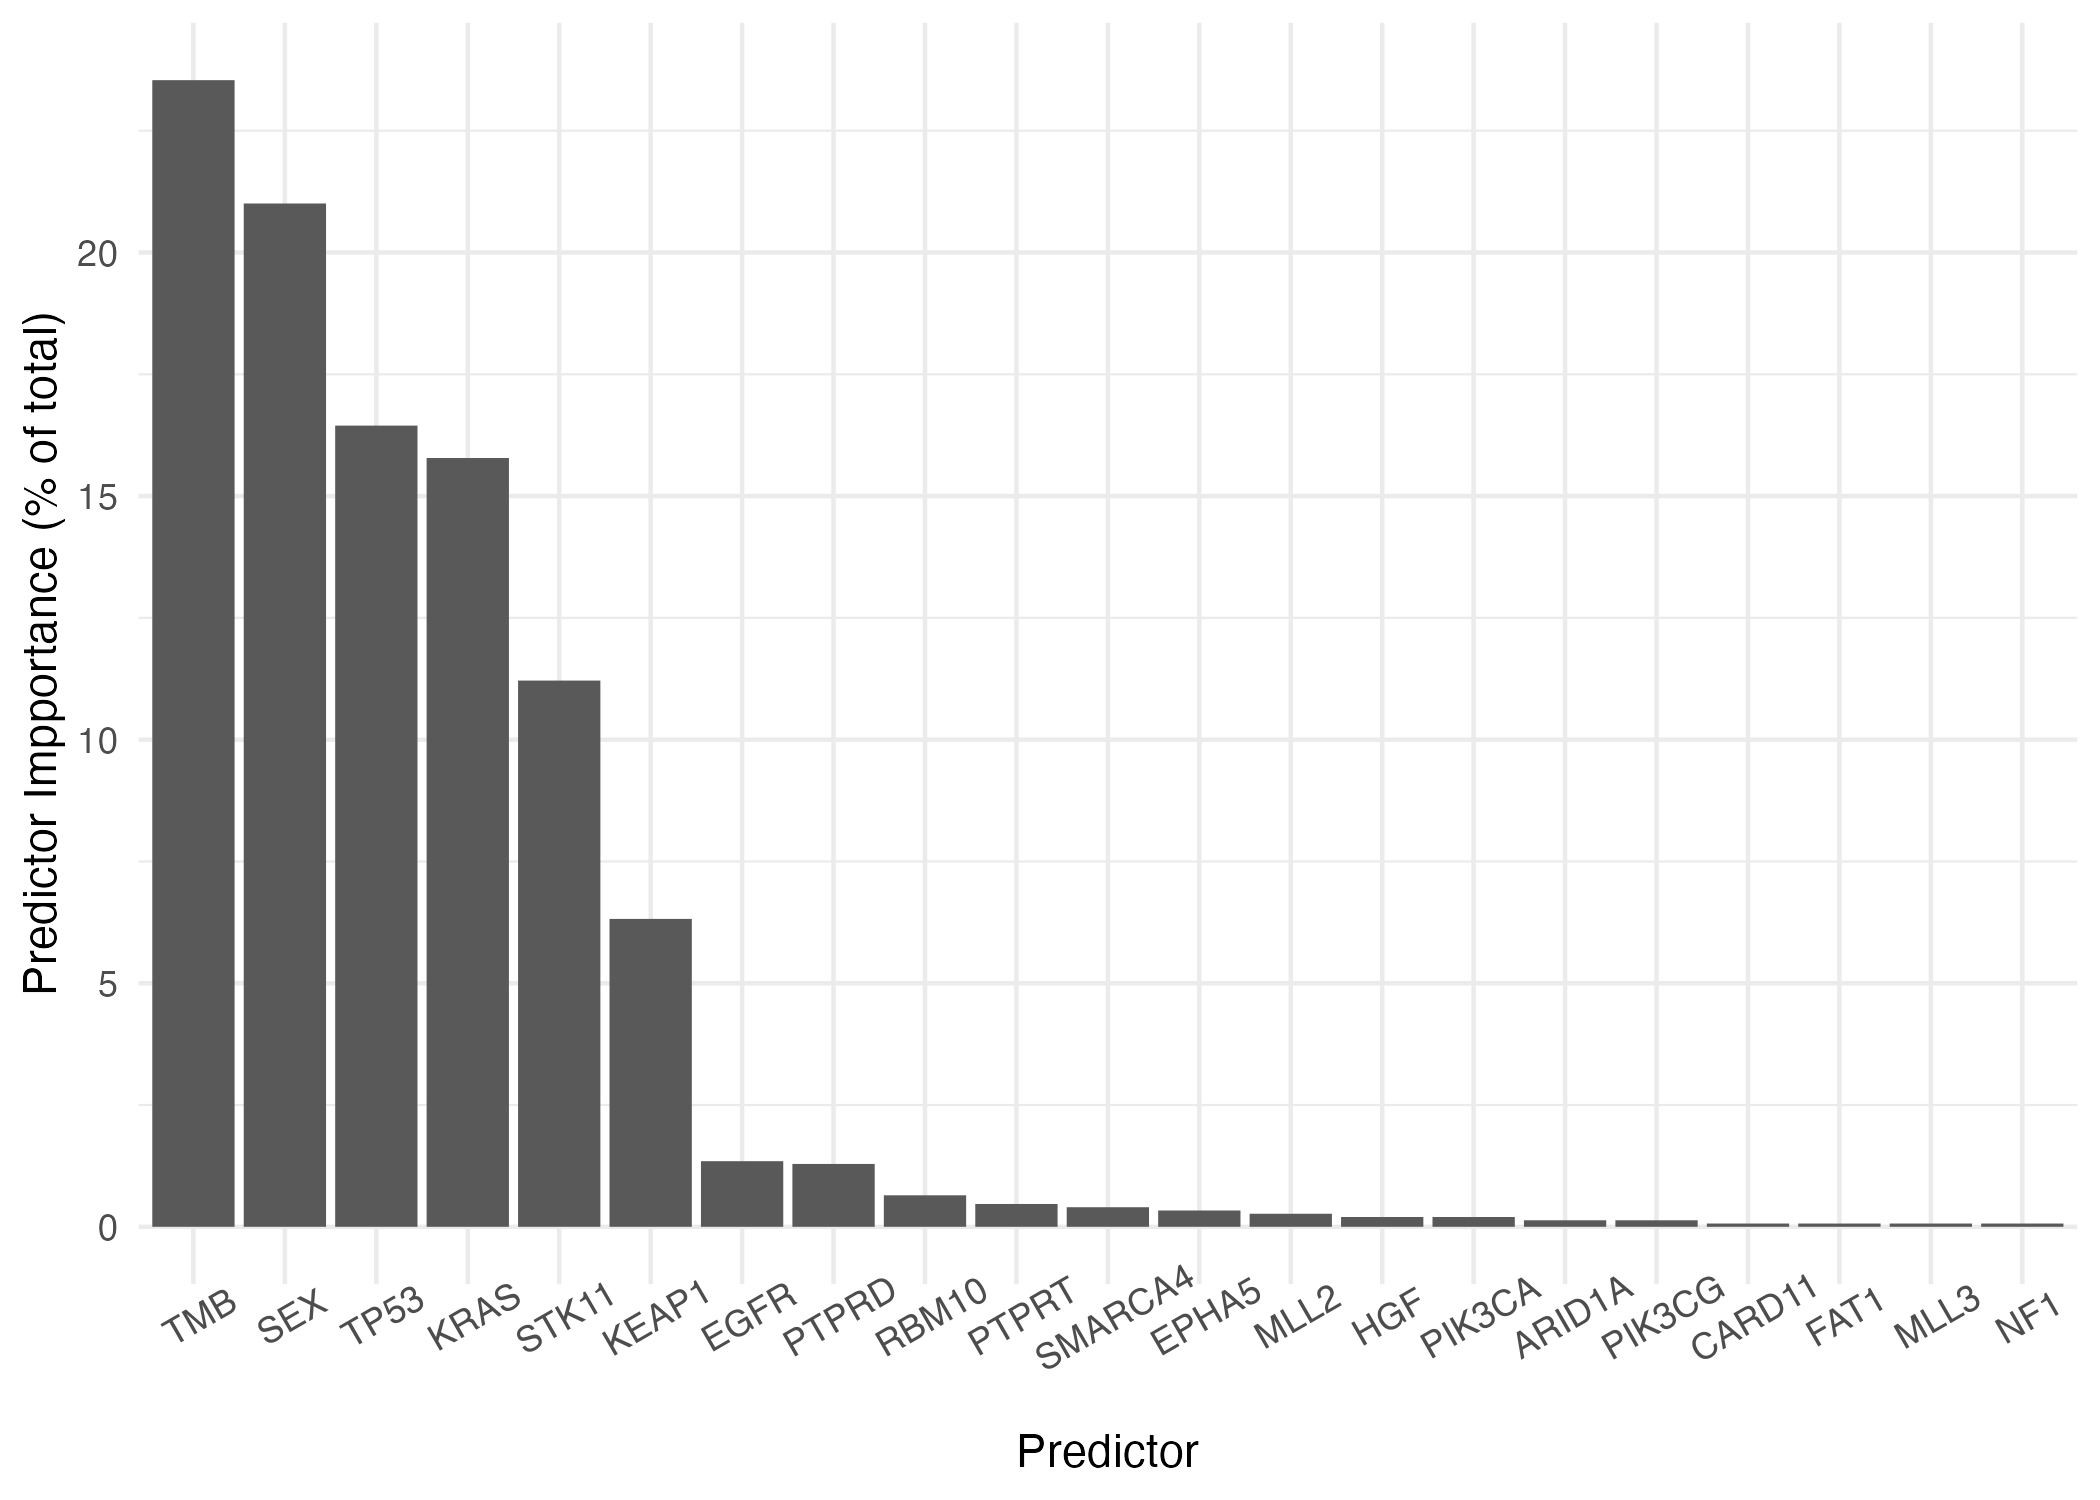
\includegraphics[width=\textwidth]{figures/chapter4/immuno_panel_variable_importance.png}
\caption{Top $\sim$20 genomic and clinical predictors of heterogeneous survival treatment effect, alongside their estimated within-forest importance metrics.  \label{fig:immuno_panel_variable_importance}}
\end{figure}

We see that, while no individual gene target is of the predictive importance of \gls{tmb} or sex in this larger combined model, but several come close. These include several usual suspects such as \emph{TP53}, \emph{KRAS}, \emph{STK11}, and \emph{KEAP1}. In order to understand the relationship between a gene's influence on the causal survival forest model and its \gls{bmr}, we compared variable importance scores with total mutation counts across the training dataset for each gene in the MSK-IMPACT panel, with outputs shown in Figure~\ref{fig:immuno_importance_vs_rate_panel}. While we observe some anomalies, such as \emph{EGFR}, we do see broadly that all highly weighted genes are those with elevated mutation rate.

\begin{figure}[!tpb] 
\centering
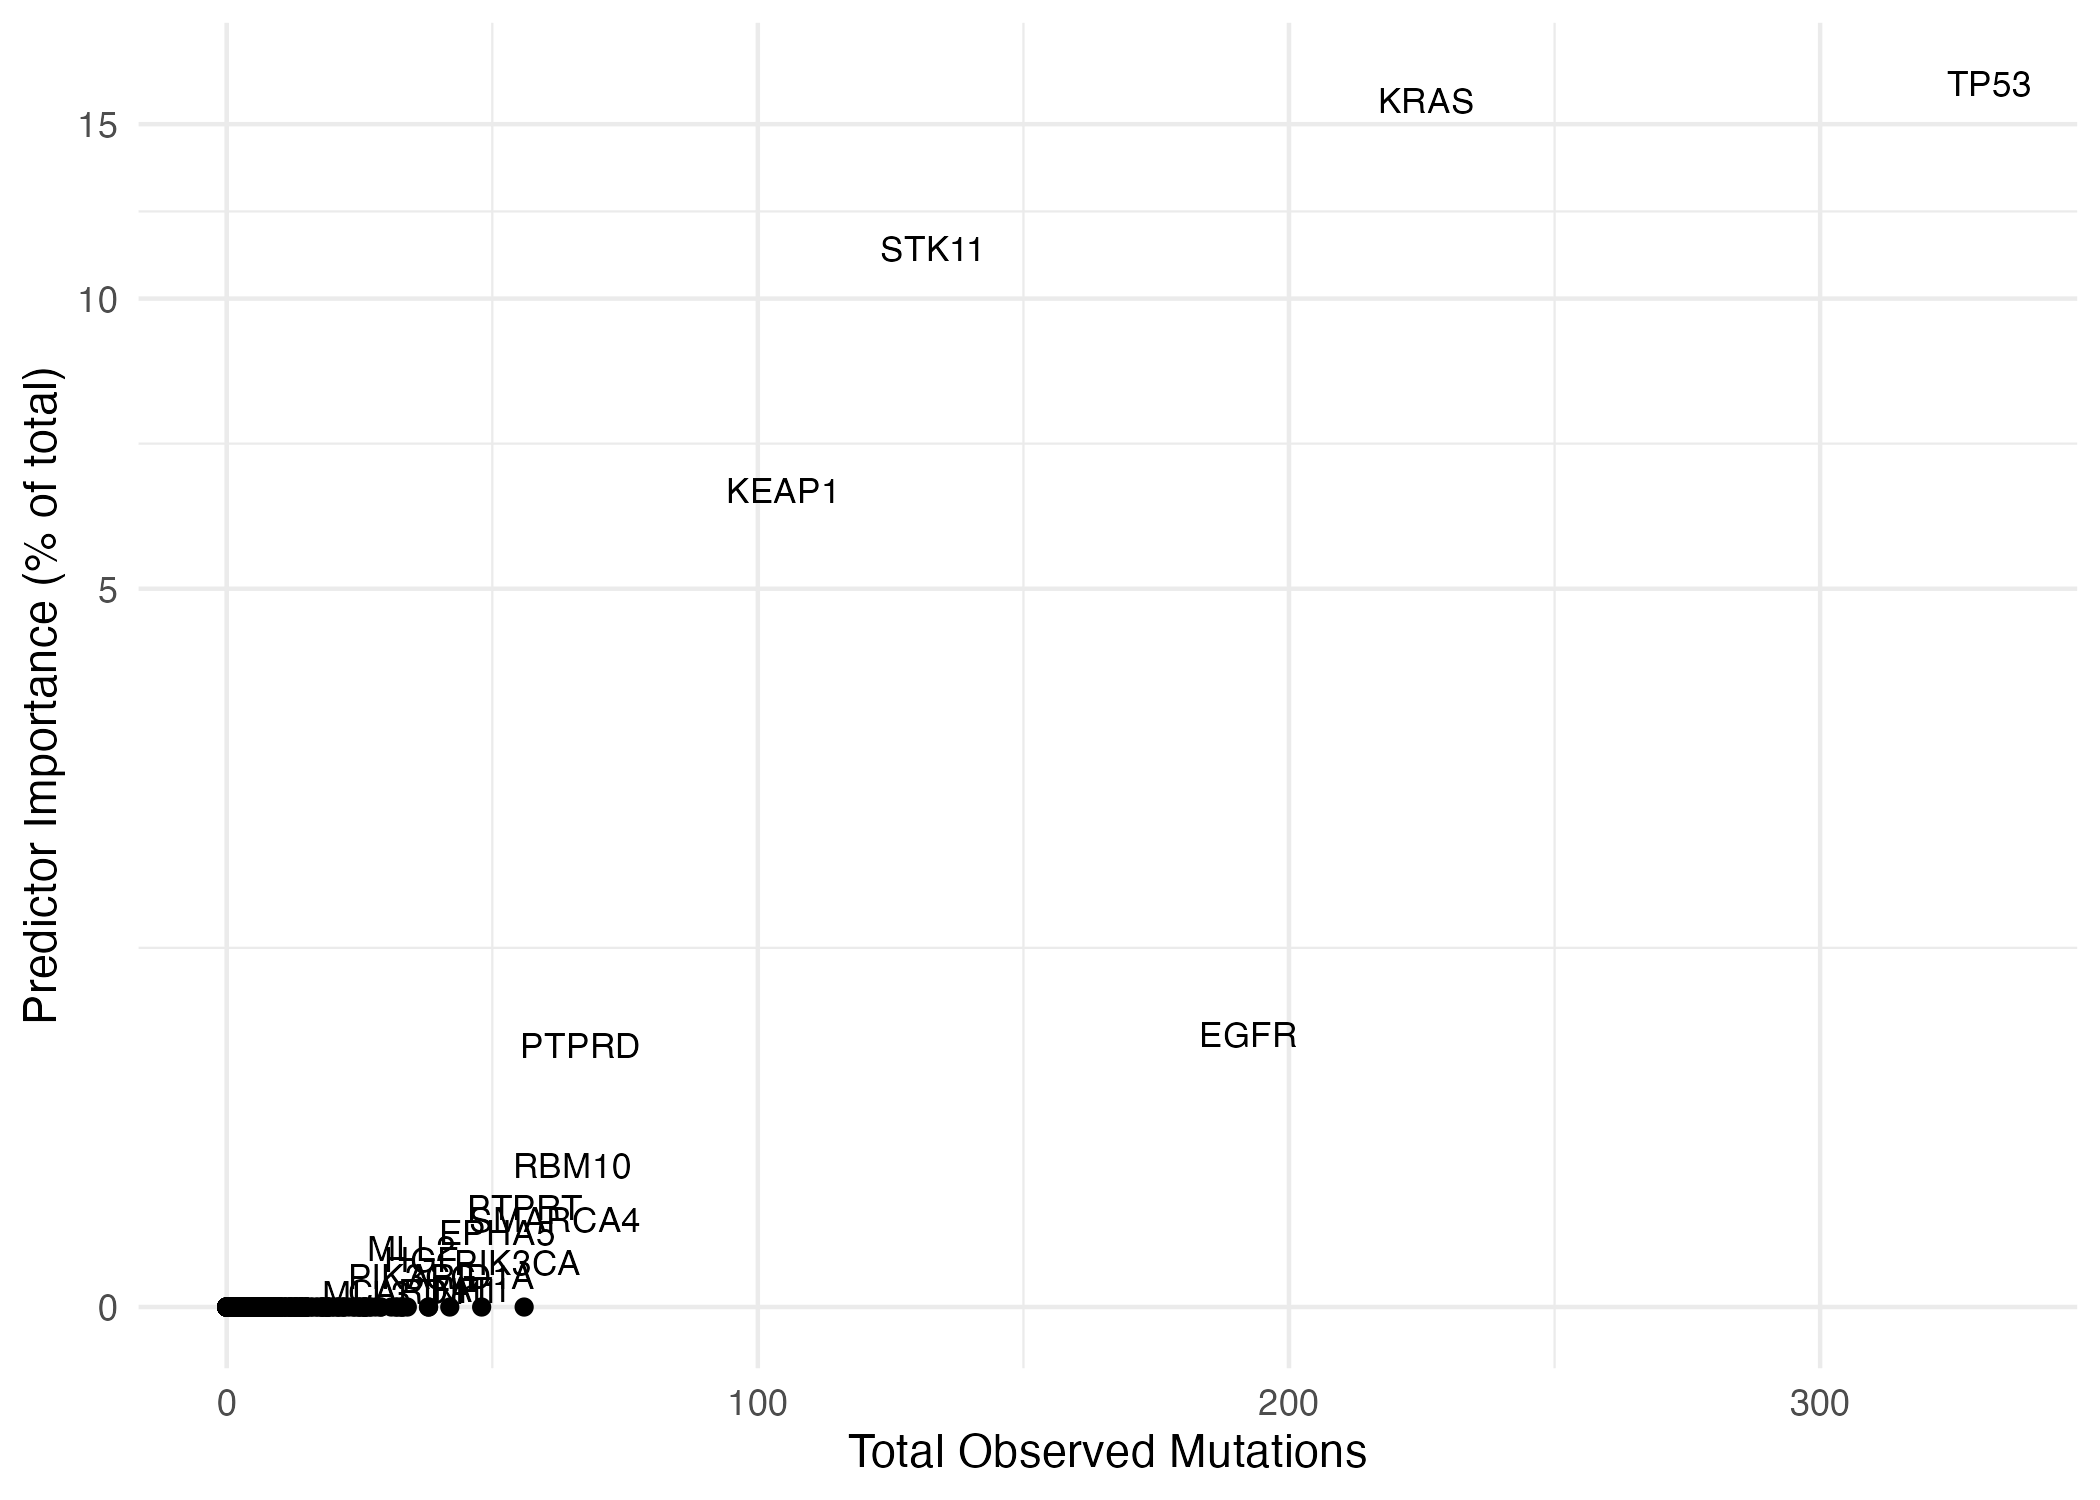
\includegraphics[width=\textwidth]{figures/chapter4/immuno_importance_vs_rate_panel.png}
\caption{Total number of mutations observed in each gene target across the training set, vs  percentage of predictive importance in the resultant causal survival forest ascribed to each target (targets with importance $>0$ labelled).  \label{fig:immuno_importance_vs_rate_panel}}
\end{figure}

\section{Conclusions}
{\color{red} \begin{itemize}
    \item Restrictions working with few clinical variables
    \item Difficulties in model validation
    \item Difficulties in application
\end{itemize}}

\dobib % renders bibliography (only when compiling for chapter only)


\end{document}